\chapter{Custom EIT Meshes}
\label{chap:chapter-5}

\emph{This work has been presented in part at: 
 the 21st International Conference on Biomedical 
 Applications of Electrical Impedance Tomography (EIT 2021)~\parencite{stowe_generating_2021}.} 

%\section*{Acknowledgement}
%\emph{Tidal Medical funded the work presented in this chapter.}

\section{Introduction}
One major challenge of EIT imaging is that the geometry of the 
external boundary where the electrodes are placed is unknown. 
Medical images of patients (such as CT images) can provide 
additional spatial information 
on patient geometry for the external boundary and location of organs. 
Recent work has shown that using a custom mesh can improve
EIT estimates of lung inhomogeneity \parencite{yang_lung_2021} in 
ARDS patients, but generating custom meshes manually is not always feasible,
and automatic segmentation of CT images is not always reliable. 
This chapter uses diagnostic CT images from 4 subjects to design and test 
a tool to create custom meshes for each patient. 
Manual segmentation of CT images can be very time consuming, 
but unsupervised automatic segmentation does not always perform reliably 
and can result in inaccurate meshes. 
In this chapter we combine automatic image 
segmentation with a manual validation stage 
to identify an accurate boundary of the body surface and lungs. 
Once the segmentation is verified, a mesh with custom lung regions is generated to 
allow for EIT reconstruction on a personalized mesh. 
A personalized mesh is expected to increase spatial accuracy 
in reconstructed EIT images. 
Higher spatial accuracy in 
identified organs and regions of interest could allow for 
easier isolation of the perfusion signal, and more accurate 
measures of perfusion and ventilation with EIT.
Motivated by the work presented by \citeauthorandyear{yang_lung_2021},
the work in this chapter focuses using custom meshes to improve measures 
of ventilation
in the lungs.  We hypothesize this might be able to  
better guide ventilation and improve treatment outcomes 
for patients with acute respiratory distress syndrome (\acrshort{ards}).

ARDS is a form of
respiratory failure caused by widespread swelling and 
accompanied by an accumulation of fluid in the 
lungs. 
ARDS is a challenging disease to diagnose and treat. 
No gold standard test exists for diagnosis, 
and few treatments are 
effective~\parencite{pham_fifty_2017}. The 
mortality rate is estimated to be as high 
as 40\%~\parencite{abe_epidemiology_2018}.
Early studies on the pathology of ARDS suggested
adjusting positive end-expiratory pressure
\acrshort{peep} to improve oxygenation in 
patients~\parencite{petty_cards_2001,ashbaugh_acute_1967}, 
and recent research suggests that treatment strategies to 
reduce lung injury during ventilation outperform
pharmacological interventions~\parencite{duggal_pharmacological_2015}. 
Monitoring ARDS patients during ventilation is vital to ensure that 
ventilator-induced lung injury is avoided~\parencite{bates_ventilator-induced_2018}, 
but few appropriate techniques are available. Computed tomography (CT) images used for
diagnosis are inappropriate for continuous use due to ionizing radiation 
exposure, and other global parameters of lung function may not give an accurate
estimate of lung homogeneity~\parencite{zhao_evaluation_2009}. 

EIT was proposed
as a monitoring technique for ARDS patients since it is non-invasive 
and can safely monitor and image the lungs in 
real time~\parencite{denai_absolute_2010,frerichs_chest_2017}.
One of the most useful parameters to classify lung ventilation 
with EIT has been global inhomogeneity (\acrshort{gi})
\parencite{sribar_influence_2020,hough_effect_2016,humphreys_effect_2011,
zhao_regional_2012,hochhausen_comparison_2019,hsu_regional_2017}.
GI has been identified as a clinically useful parameter to monitor 
ventilation~\parencite{frerichs_chest_2019}.

The largest issue with using EIT for regional 
ventilation monitoring is that incorrectly modelling the 
boundary can introduce large artefacts in reconstructed
images~\parencite{grychtol_impact_2012}. The correct 
lung boundary is also required to calculate metrics like GI
index~\parencite{zhao_evaluation_2009}.
Incorrectly modelling the boundary and lung area when investigating 
regional homogeneity can also lead to an incorrect GI 
estimate \parencite{yang_lung_2021}. 
\citeauthorandyear{yang_lung_2021} found that 
a mesh with custom segmented external and lung boundaries 
was more sensitive to changes in lung condition using GI 
compared with generic models.
This suggests a custom mesh with more defined lung regions 
may also improve sensitivity to lung-based pulsatility and 
improve measures of perfusion. 
While GI index is a valuable parameter, it does not 
give a direct indication of the spatial information in EIT reconstructions.
In this chapter the centre of ventilation is used instead 
to compare between EIT recordings and the ventilated region extracted
from CT images. This metric is used to determine if 
a ventilation parameter measured on a custom mesh can be more accurate than 
when generic meshes are used.

Custom meshes have been created by segmenting the boundaries of lungs and organs
to monitor ARDS \parencite{yang_lung_2021}, but automatic segmentation of the lung region 
for a large number of ARDS patients is a challenging problem. Typically, ARDS patients 
will have a combination of
lung swelling, fluid build-up in the lungs, and lung collapse; this
obscures the 
true boundary of the lungs. \Fref{fig:raw-ct} depicts unprocessed CT slices 
of the 4\textsuperscript{th} intercostal space from 4 subjects with
ARDS. This figure highlights the challenges  of automatically 
segmenting lung tissue across several subjects. 
In some CT images, the arms obscure the external boundary; in 
others, partial or total occlusions 
mask the true lung boundary.

\begin{figure}[H]
	\centering
	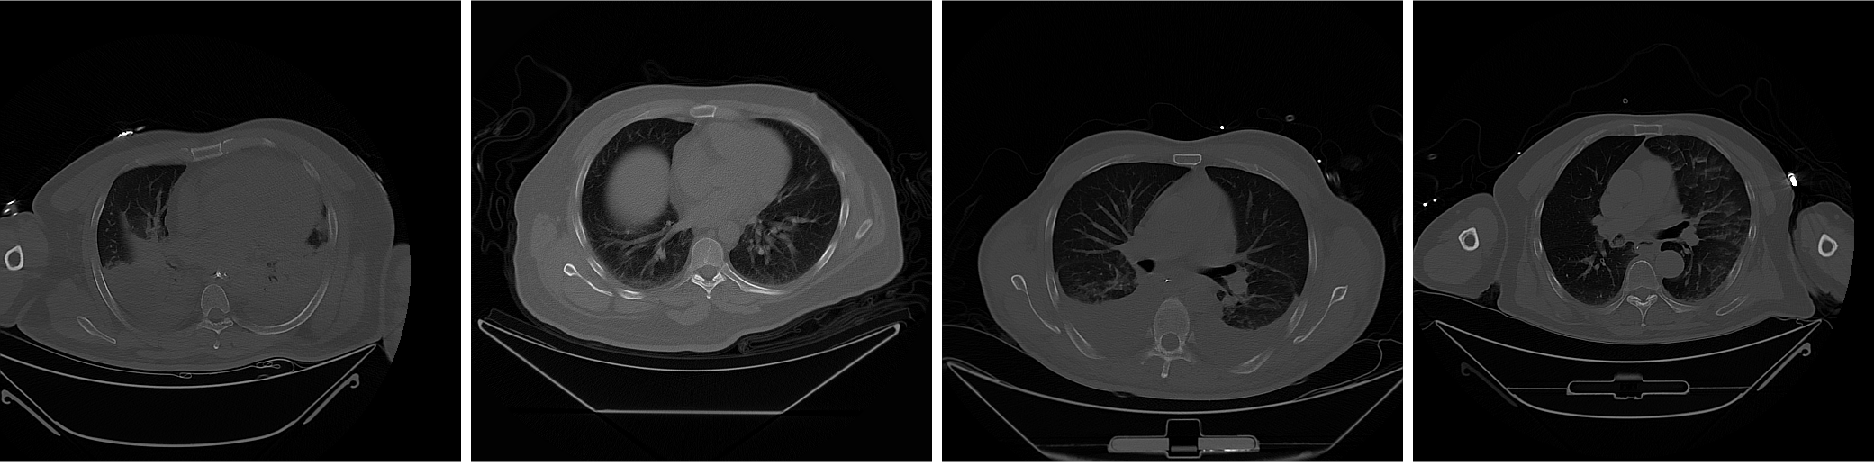
\includegraphics[width=\textwidth]{chapter5-CT_to_mesh/imgs/raw_ct_imgs.png}
	\caption[Raw CT images at the 4\textsuperscript{th} intersoctal space]{\label{fig:raw-ct}%
	This figure shows raw CT data from 4 subjects  taken at the 4\textsuperscript{th} intercostal space.
	These images highlight the challenges with automatic segmentation of the lung and external boundary. 
	In some subjects the external boundary is obscured by the arms, and in other subjects the 
	true lung boundary is masked by occlusions.
	}
\end{figure}

This chapter introduces a tool that enables automatic segmentation 
of the lungs and exterior boundary, with manual correction to facilitate individualized
bedside monitoring and guide treatment of ARDS.
This tool processes and automatically segments the external and lung boundaries 
in diagnostic CT images, 
then presents them for manual correction 
to create custom EIT models. 
The goal of this chapter is to generate custom models that improve reconstruction 
accuracy
in the lung regions. 
These models may facilitate real time, individualized ventilation
monitoring for ARDS patients.  

\section{Methods}
This section presents the methodology for:
\begin{itemize}
	\item Automatic segmentation of diagnostic CT images (\fref{sec:auto-segment})
	\item Design of a manual segmentation correction tool (\fref{sec:correct-segment})
	\item Mesh generation (\fref{sec:mesh-gen})
	\item Comparison of ventilation centre of mass 
	between generic and custom EIT models (\fref{sec:gi-scores})
\end{itemize}

\begin{figure}[H]
	\centering
	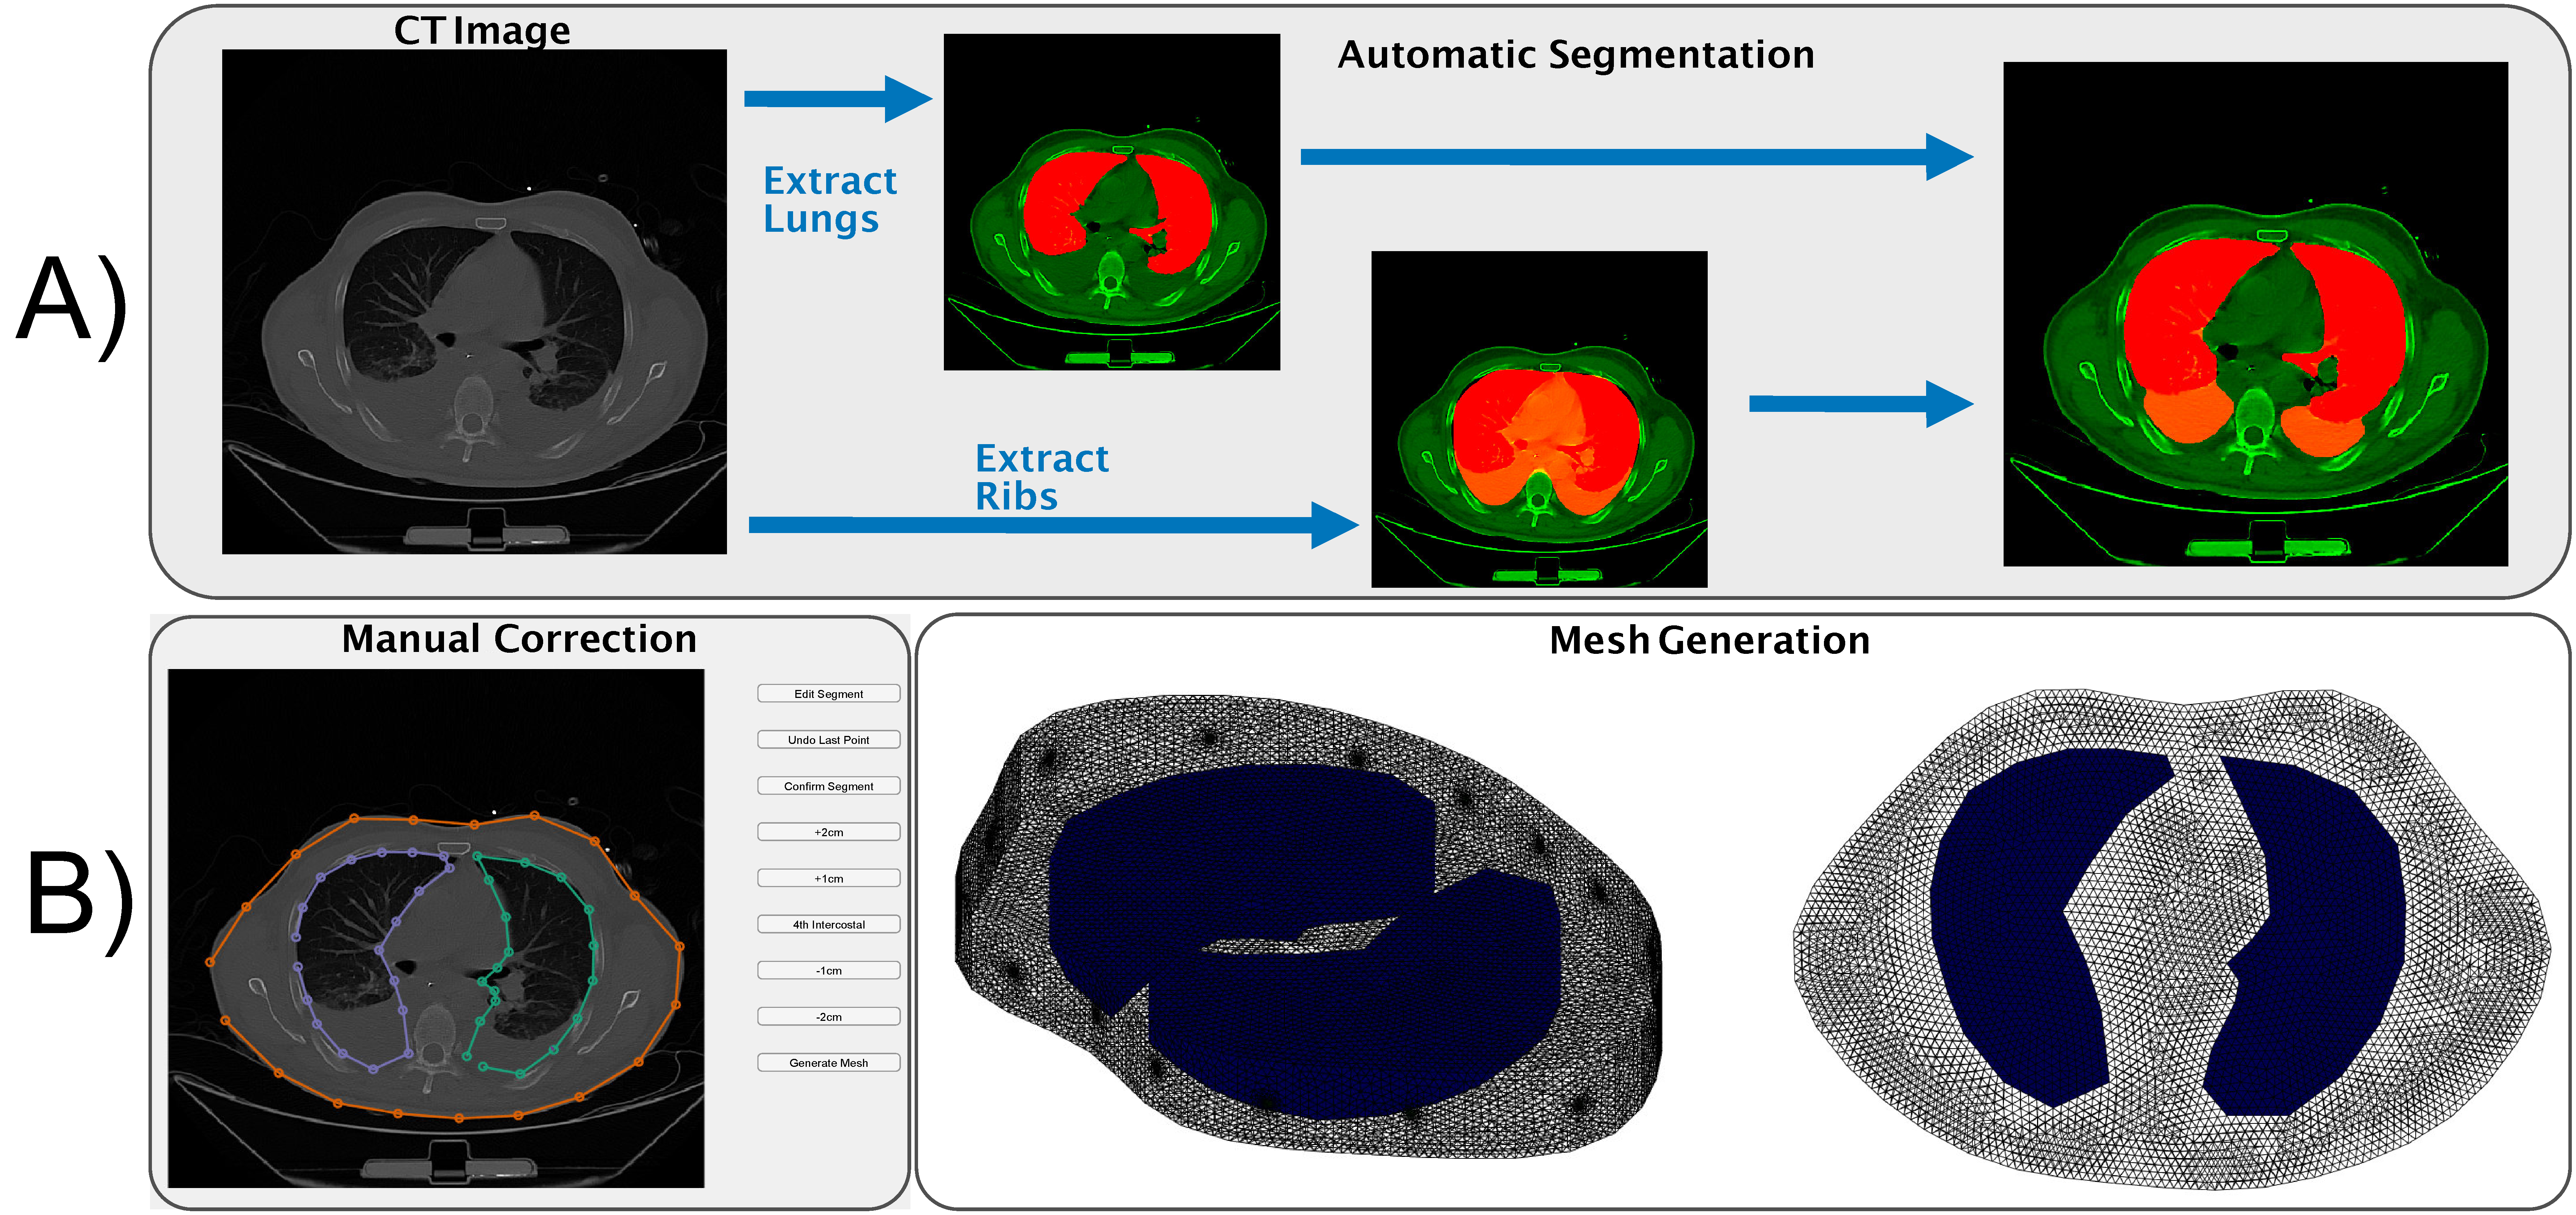
\includegraphics[width=\textwidth]{chapter5-CT_to_mesh/imgs/methods_figure.pdf}
	\caption[Mesh generation method overiew.]{\label{fig:segment_overview}%
	An overview of the segmentation and editing process showing: 
	A) A sample raw CT which was thresholded, scaled and adjusted over several 
	adjacent slices to identify
	the lung regions and an enclosed rib area, and the resulting lung estimate; and
	B) A screen  capture of the manual mesh correction process and 2 views of the generated
	mesh.
	}
\end{figure}

\Fref{fig:segment_overview} shows a summary of the mesh generation process from raw diagnostic CT 
data to a custom mesh based on the geometry of the patient.
First, CT images are acquired and automatically segmented. Then they are verified or corrected, and a custom mesh is created.
Matlab 2021a (Mathworks, USA) with the 
image-processing toolbox was used for the image segmentation and manual correction interface.
Mesh generation and reconstruction was performed with 
EIDORS 3.10~\parencite{adler_eidors_2017} using Matlab 2019b.
At the time of writing Matlab 2019b was required to 
use certain EIDORS functionality, but Matlab 2021a provided some additional 
features that improved responsiveness of the 
graphical user interface \acrshort{gui}.

\subsection{Automatic Segmentation of the Thorax} \label{sec:auto-segment}
Automatic segmentation of lung regions in ARDS patients is challenging due to the variability
in lung tissue intensity, and the presence of fluid or collapsed lung regions. 
In some patients the lung regions were not visible in the image and even manual
correction of the segmentation required approximation. 
This project uses an automatic technique to identify the chest cavity using several adjacent vertical CT images to
locate the ribs.
Even when no lung is visible in the image, this produces a starting point
close to the expected boundary which reduces correction time. 
This tool is designed to approximate the true lung boundary as closely as possible to 
simplify manual correction if the lungs cannot be segmented.
If no ribs or lung are detected, ellipses are placed within the boundary 
close to the expected lung location that 
can be corrected manually.

The automatic segmentation step uses a diagnostic CT image 
with the slice corresponding to the 4\textsuperscript{th} intercostal space 
identified. 
To begin segmentation, the user must select the series of CT images they 
wish to segment, and the frame number that corresponds to the 4th intercostal 
space. For the 4 test subjects, the 4\textsuperscript{th} 
intercostal space was identified manually using
3D Slicer 4~\parencite{fedorov_3d_2012}. 
This location corresponded to the electrode belt placement for EIT measurements.

A detailed algorithmic outline of the automatic segmentation process is 
presented in \fref{app:appendix-algos}.

\subsubsection{External Boundary} \label{sec:ext_seg}
The boundary segmentation steps are shown in \fref{fig:ext_seg_methods}.
To segment the boundary, the selected raw CT slice 
(A in \fref{fig:ext_seg_methods}) 
was adjusted so that the
intensity of the lung tissue was 0 and the maximum image value was 1 
(B in \fref{fig:ext_seg_methods}). 
Next the image was eroded and reconstructed 
to remove small features and retain large structures 
(C in \fref{fig:ext_seg_methods}).
Finally, the image was binarized using a threshold of 0.5 (D in \fref{fig:ext_seg_methods}),
and holes were filled (E in \fref{fig:ext_seg_methods}), 
to give the final boundary (F in \fref{fig:ext_seg_methods}).

\begin{figure}[H]
	\centering
	% Use the following line with your images (pdf preferred)
	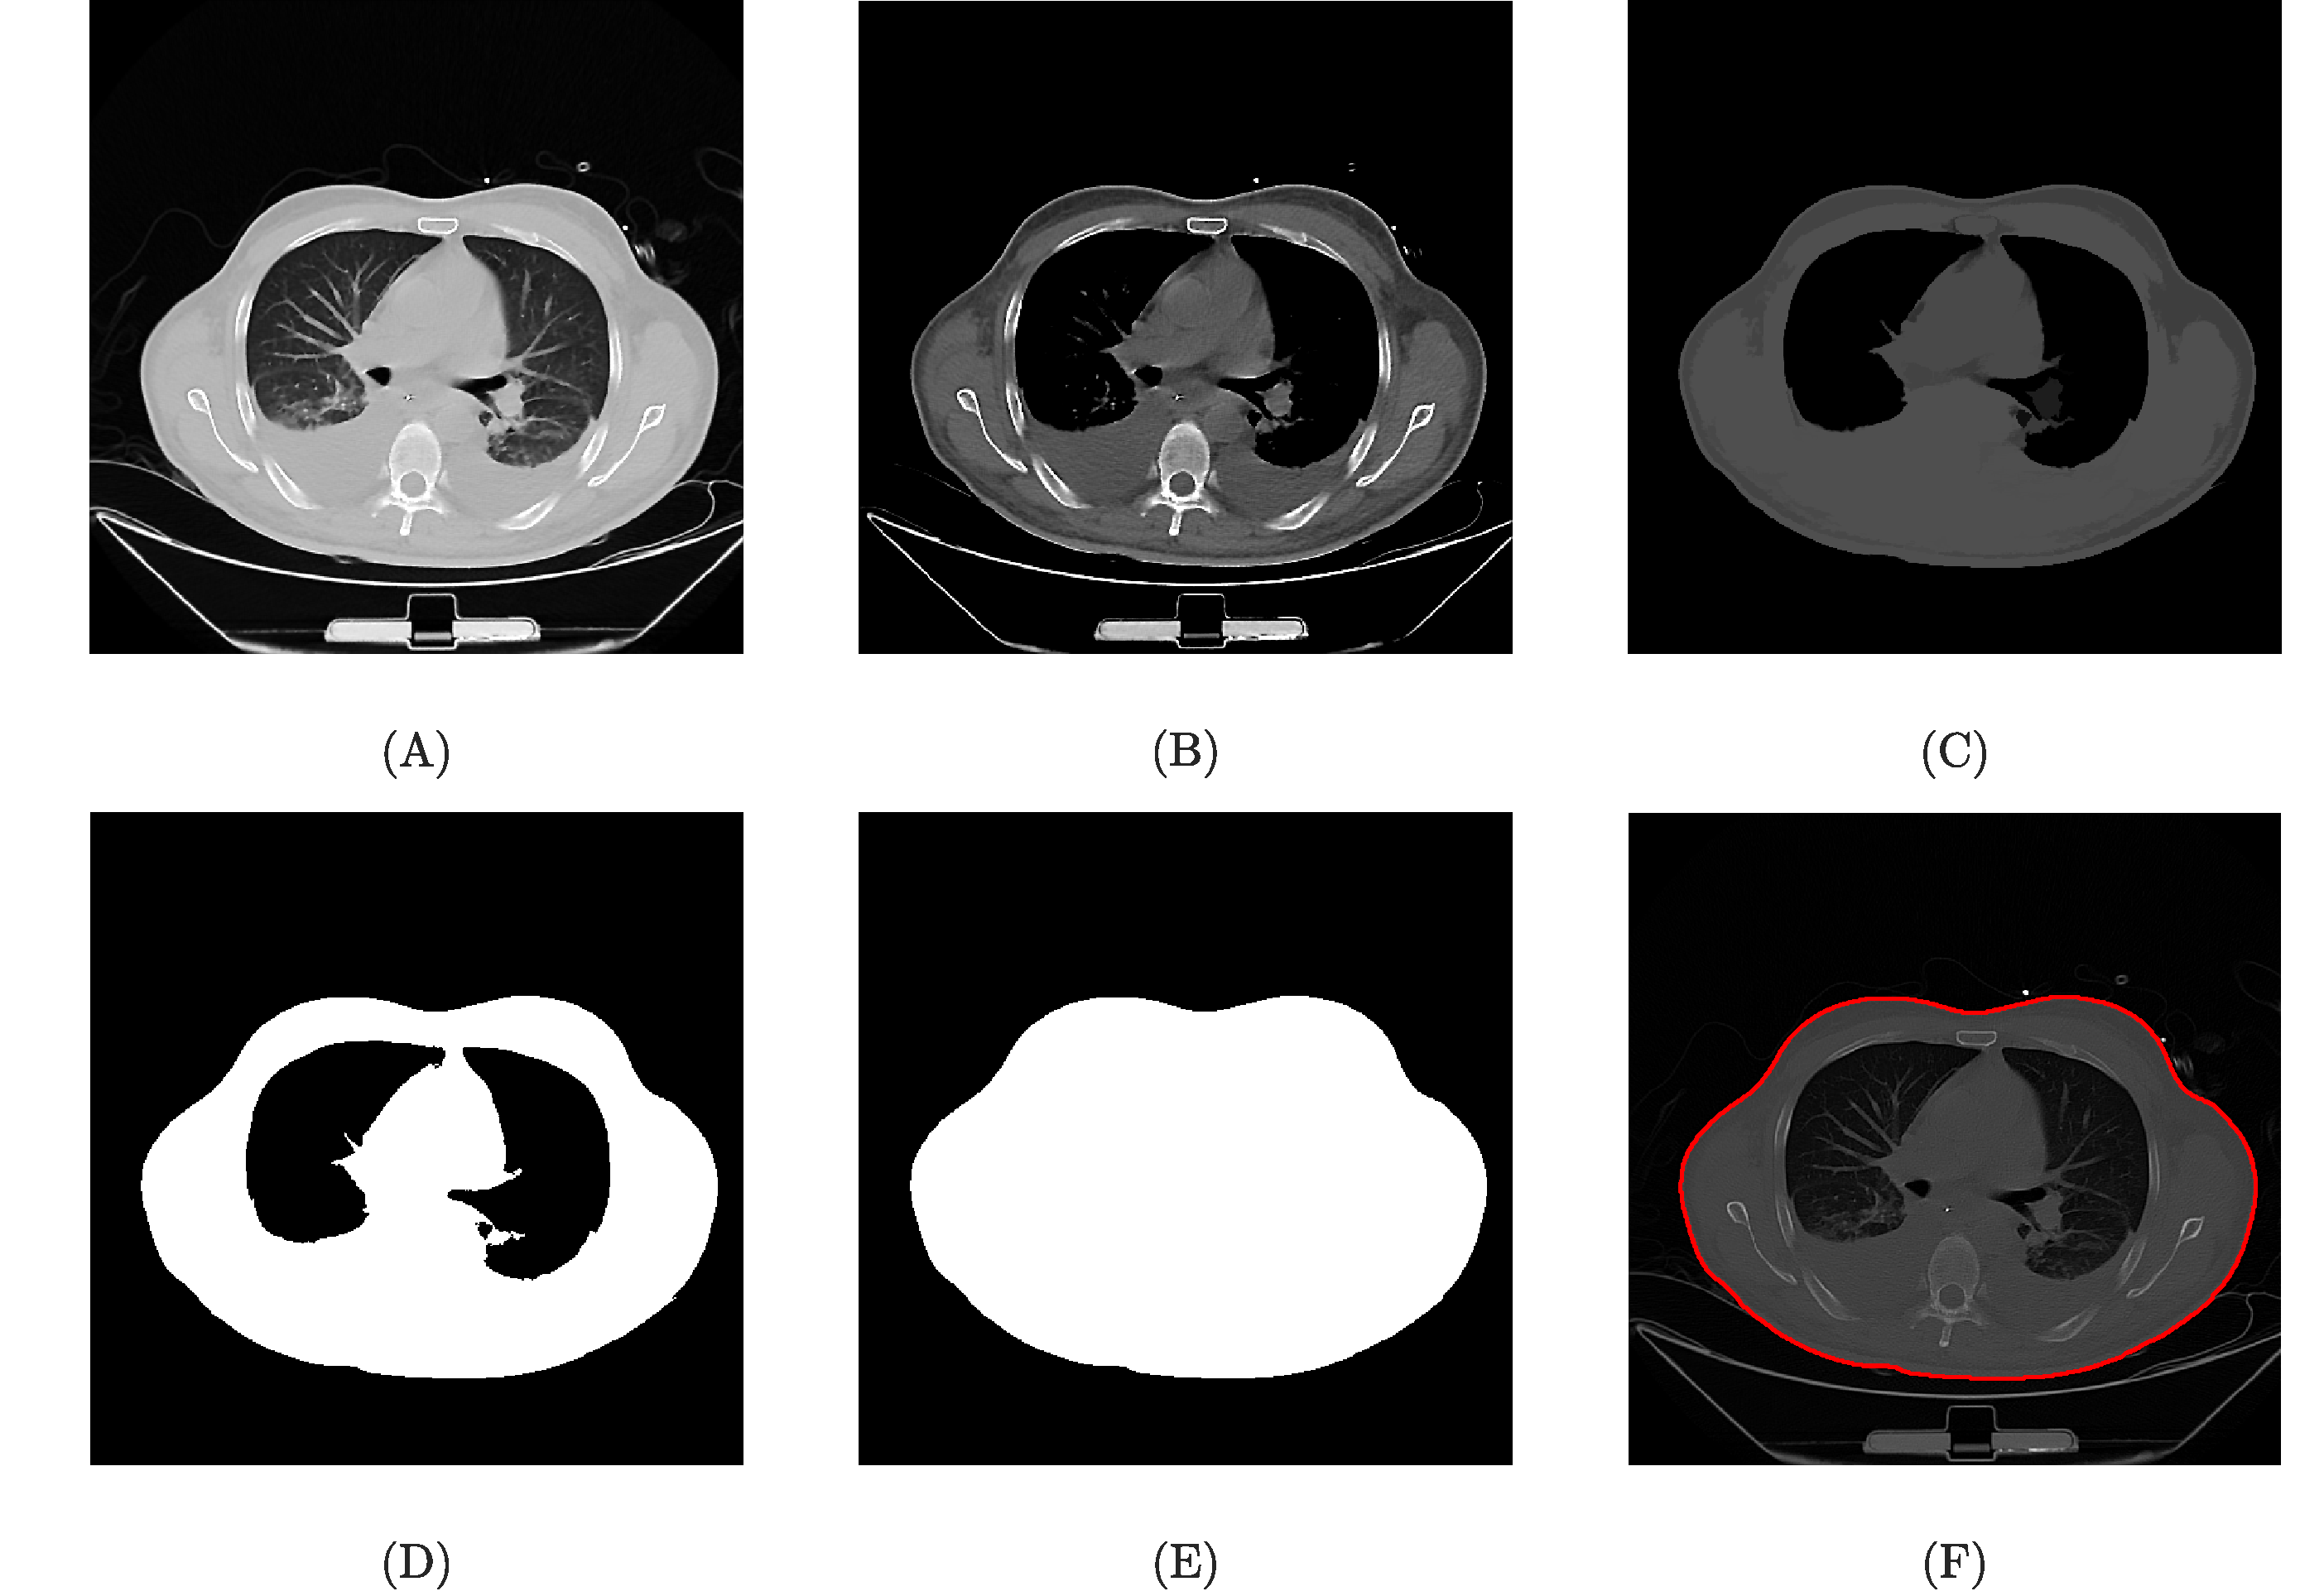
\includegraphics[width=\textwidth]{chapter5-CT_to_mesh/imgs/boundary_seg_methods.pdf}
	\caption[Boundary segmentation methods.]{\label{fig:ext_seg_methods}%
	This figure presents the external boundary segmentation process. First,
	a raw CT image of the 4th intercostal slice (A) 
	was adjusted based on the lung density (B), 
	eroded and reconstructed (C), then binarized (D) and 
	filled to give the final boundary (F).
	}
\end{figure}

\subsubsection{Chest Cavity}
To segment the chest cavity, 7 slices above and below the 4\textsuperscript{th}
intercostal space were used, giving 15 slices to segment. 
To begin, the external boundary of the selected slice was
used (segmented using the method in \fref{sec:ext_seg}). 
The initial boundary 
(A in \fref{fig:cav_seg_methods})
was eroded to form a mask from the shrunken boundary shape
(B in \fref{fig:cav_seg_methods}).
This mask was used on a binarized image (threshold of 0.5) to extract bones and bright objects from
within the thorax 
(C in \fref{fig:cav_seg_methods}).
The image was closed to fill  holes and identify bones
(D in \fref{fig:cav_seg_methods}).
Next all 15 adjacent slices were superimposed to combine all rib locations
that occurred in more than one slice
(E in \fref{fig:cav_seg_methods}).
To fill holes in the ribcage, a rectangular 
element with a height of 5 pixels and width of 50 pixels was used to close 
the top half of the image
(F in \fref{fig:cav_seg_methods}).
A final thickening operation was performed to ensure continuity
(G in \fref{fig:cav_seg_methods}).
All objects connected to the boundary were removed 
to give the final chest cavity segmentation
(H in \fref{fig:cav_seg_methods}).

\begin{figure}[H]
	\centering
	% Use the following line with your images (pdf preferred)
	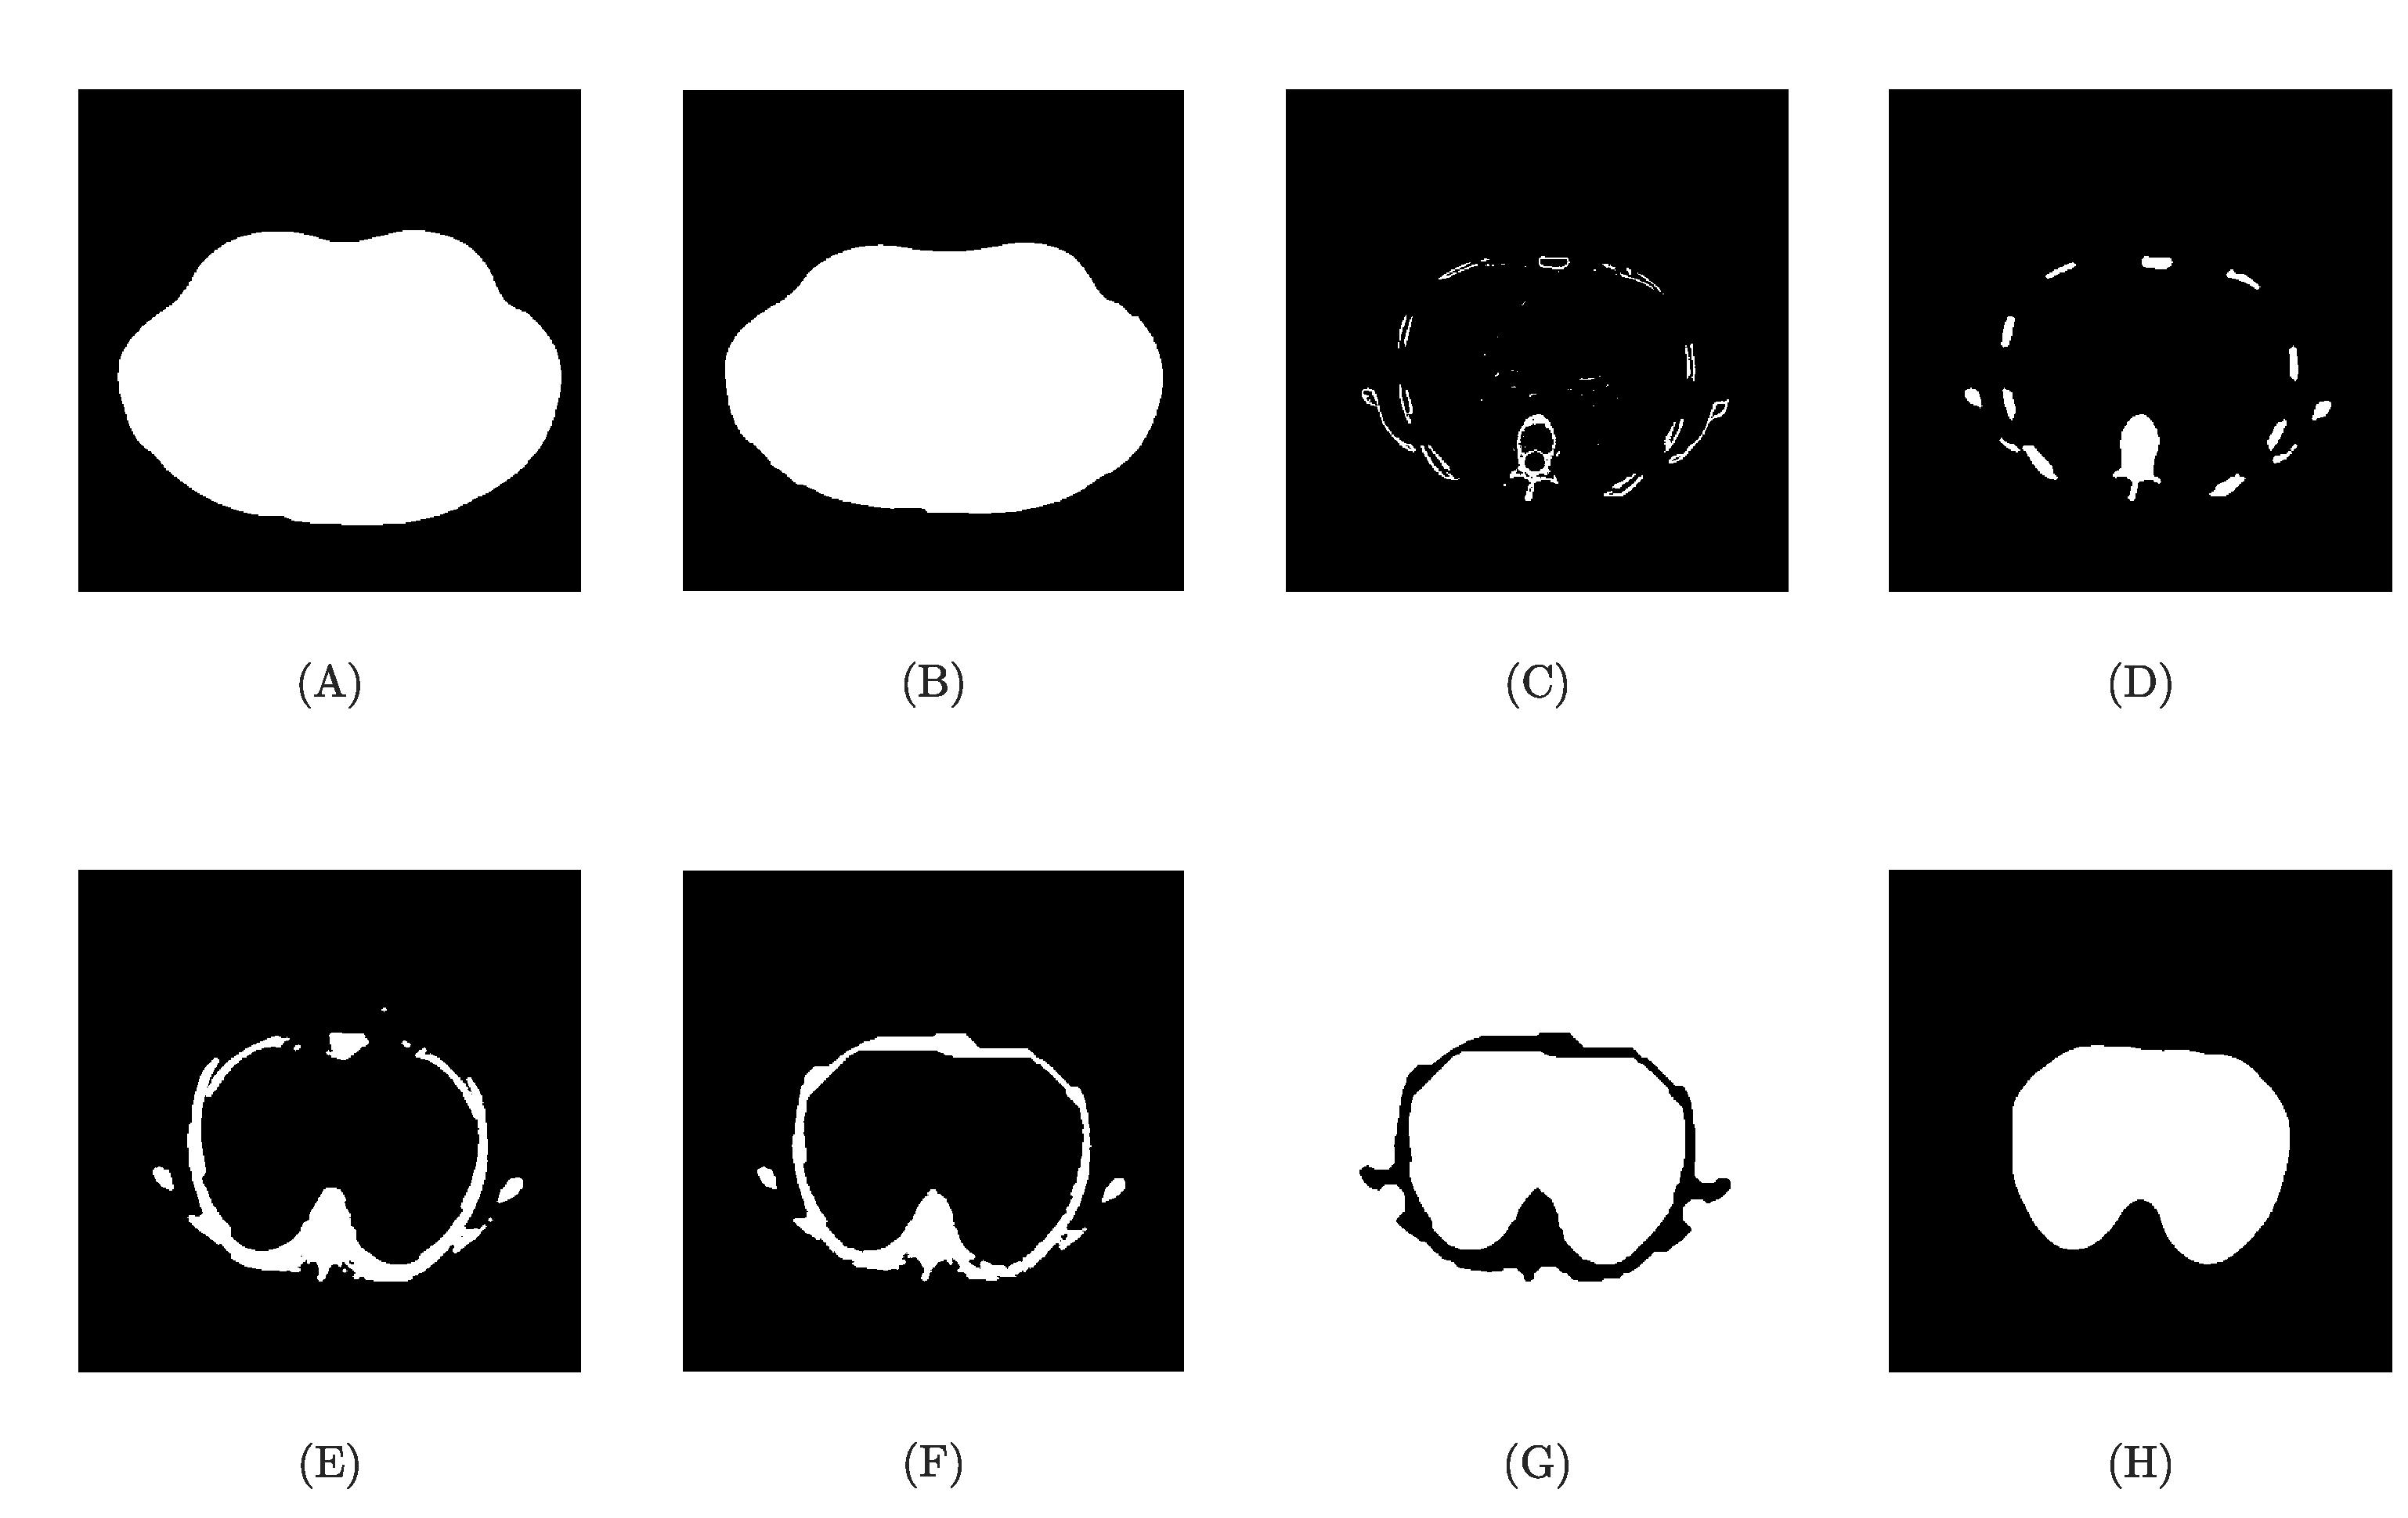
\includegraphics[width=\textwidth]{chapter5-CT_to_mesh/imgs/chest_cavity_seg_methods.pdf}
	\caption[Chest cavity segmentation methods.]{\label{fig:cav_seg_methods}%
	The chest cavity segmentation process. For each of the 15 selected slices the initial external boundary (A)
	was eroded to form a mask from the shrunken boundary shape
	(B). This mask was used on a binarized image to extract bones and bright objects from
	within the thorax (C). The image was closed to fill  holes and identify bones
	(D). Next all 15 adjacent slices were superimposed to combine all rib locations
	that occurred in more than one slice (E).
	To fill holes, a rectangular element with a height of 5 pixels and width of 50 pixels was used to close 
	the top half of the image (F).
	A final thickening operation was performed to ensure continuity
	(G). All objects connected to the boundary were removed 
	to give the final chest cavity segmentation (H).
	}
\end{figure}


\subsubsection{Lungs}
The lung segmentation was required to work in patients with ARDS and give 
an approximate lung boundary when the lungs were potentially collapsed or filled with 
fluid. To achieve this, a rough lung estimate based on the chest cavity  
was used together with a segmentation of the 
ventilated lung.
The segmentation process started with a segmentation of the chest cavity (A in \fref{fig:lung_seg_methods}).
First, an estimation of the lung region was made by placing an ellipse
in the centre of the chest cavity segmentation at the thinnest central
point (B in \fref{fig:lung_seg_methods}). Next a ventilated lung estimate 
(C in \fref{fig:lung_seg_methods})
was made
by inverting the binarized image from the external boundary segmentation
(D in \fref{fig:ext_seg_methods}). 
Finally, a complete lung segmentation was generated by removing any part of the
simple lung estimate (B in \fref{fig:lung_seg_methods}) that was within 5 
pixels of the ventilated lung region, and combining the two 
lung estimates with a closing operation. 
This produced a close estimate of the lung boundary even in cases where
little or no lung tissue was visually distinguishable. 

\begin{figure}[H]
	\centering
	% Use the following line with your images (pdf preferred)
	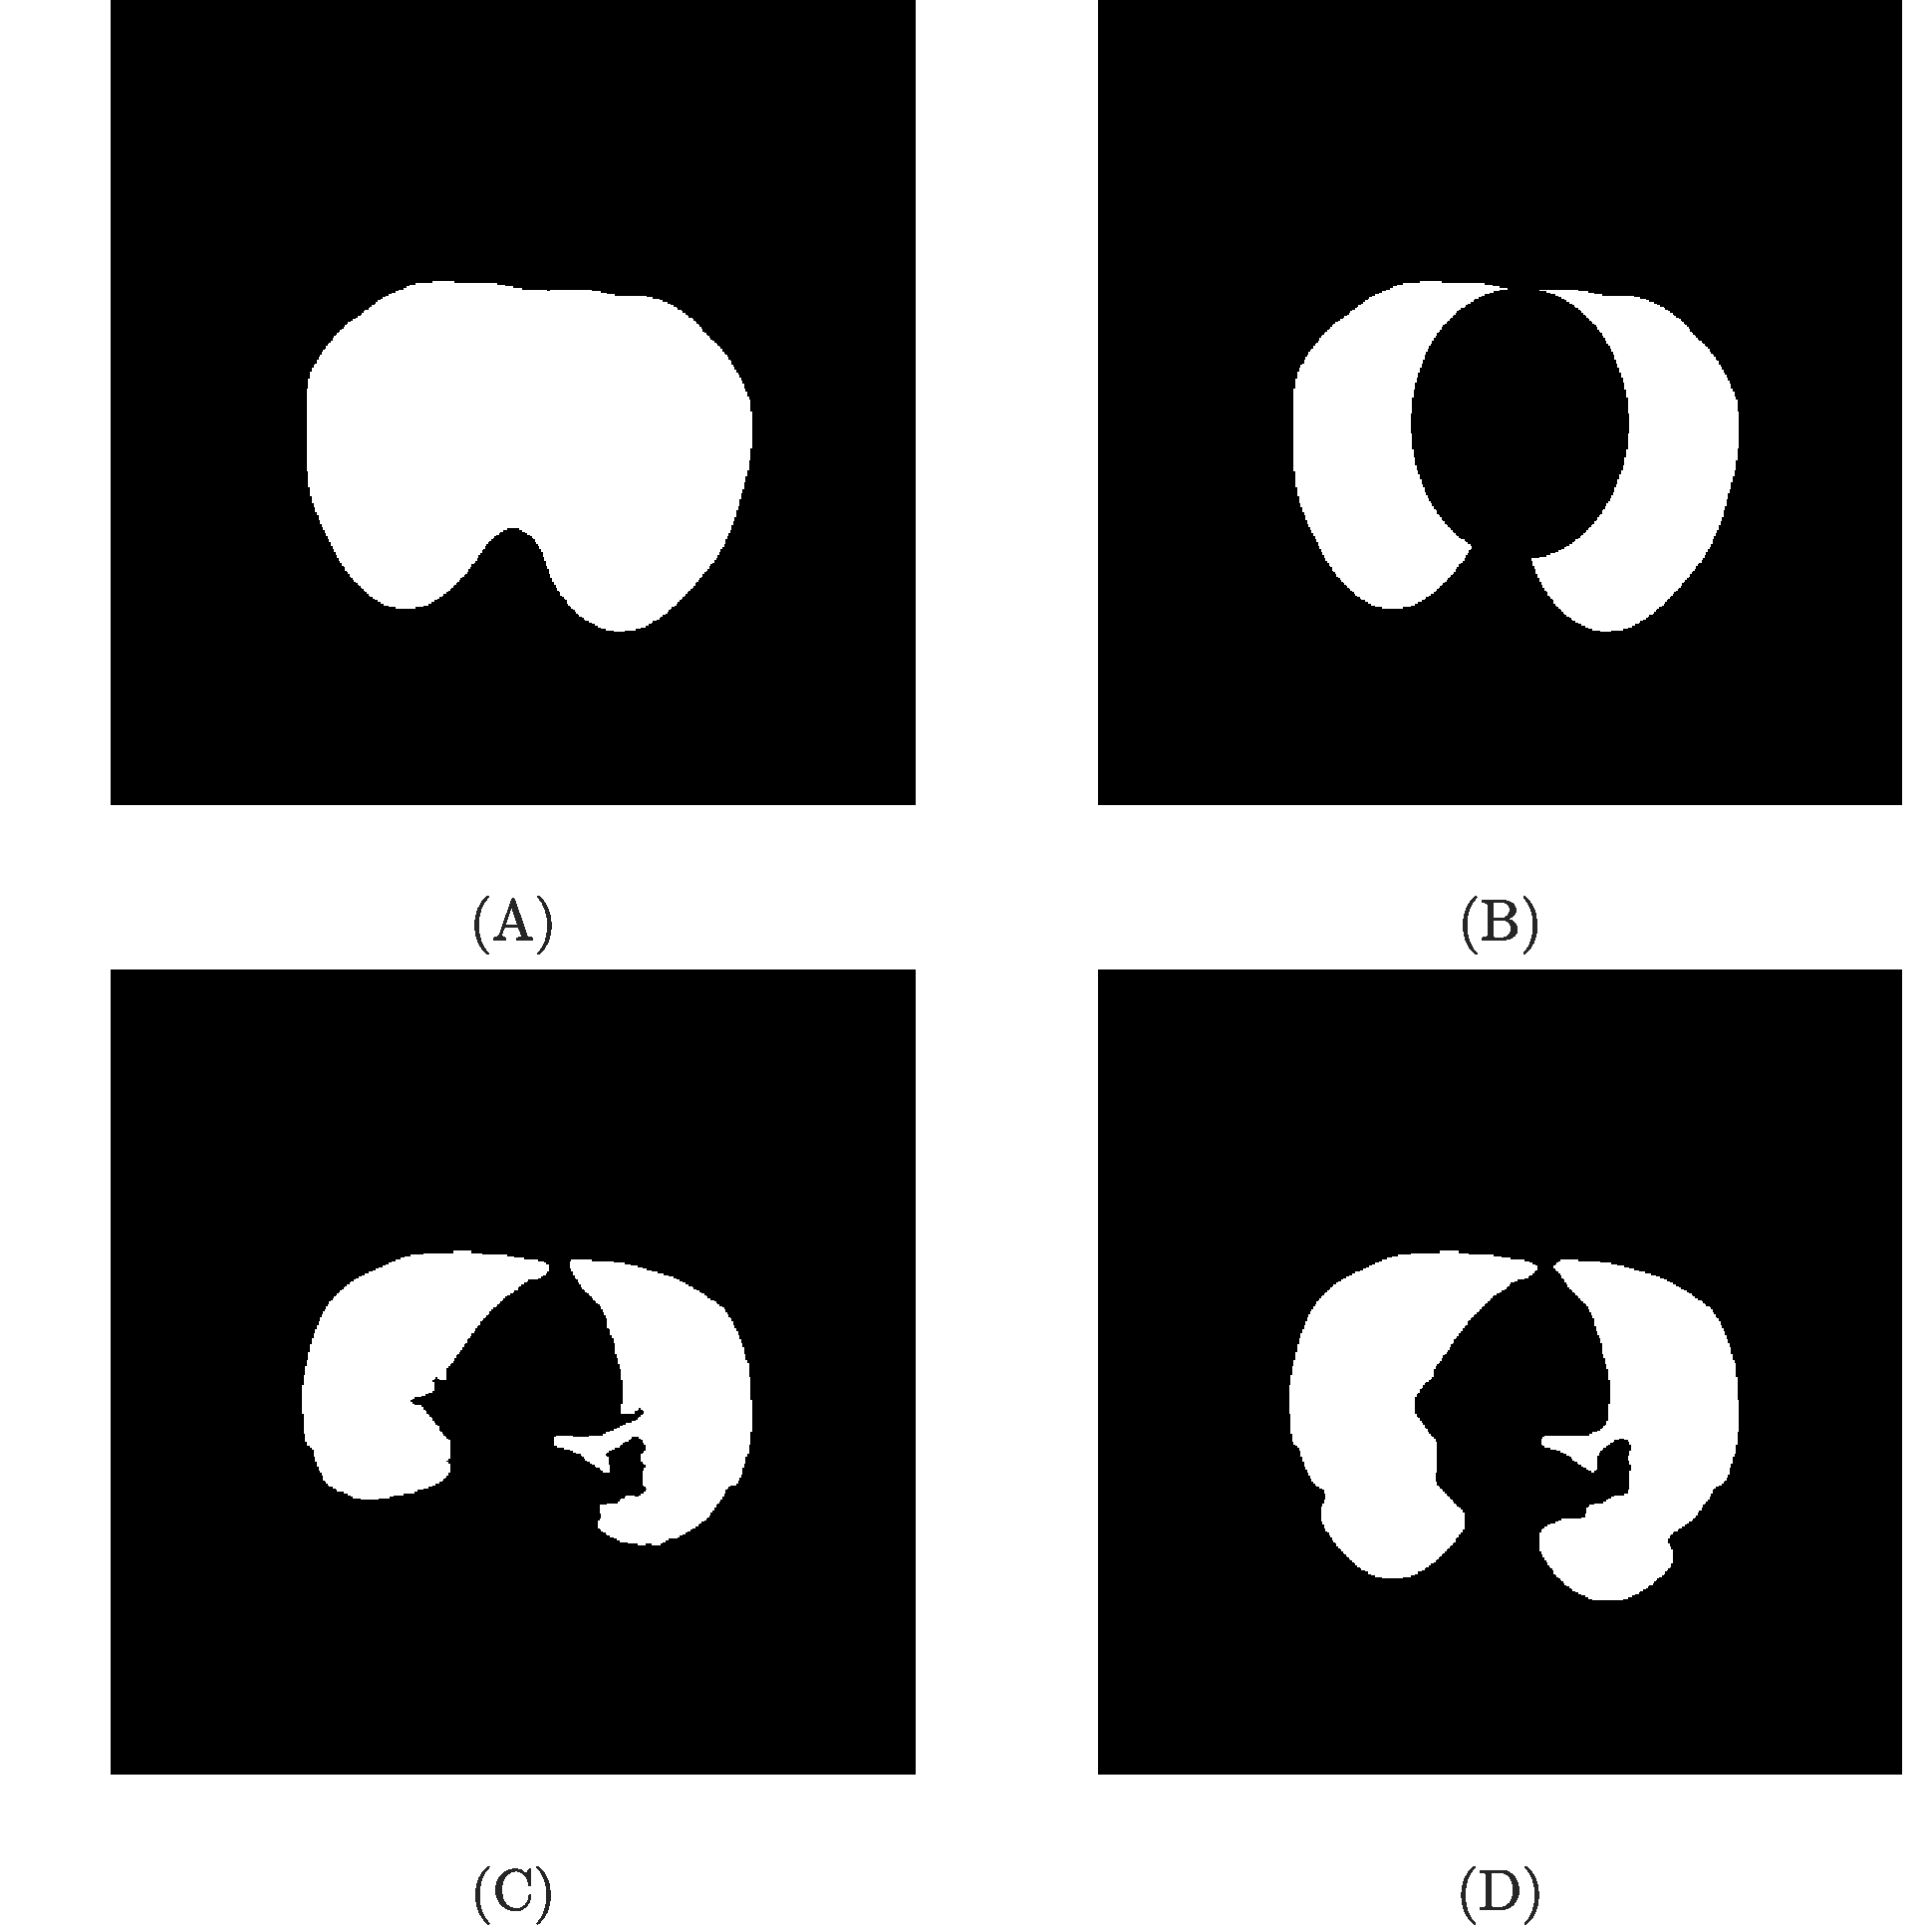
\includegraphics[width=\textwidth]{chapter5-CT_to_mesh/imgs/lung_seg_methods.pdf}
	\caption[Lung segmentation methods.]{\label{fig:lung_seg_methods}%
	The figure shows the lung segmentation methods.
	An approximation of the lung boundary was generated using the chest cavity segmentation
	(A) with an ellipse to remove the heart region (B).
	This was combined with a segmentation of the ventilated lung region (C) 
	to give a total lung estimate (D).
	}
\end{figure}

\subsection{Manual Segmentation Correction}  \label{sec:correct-segment}
Although the automatic segmentation was carefully designed to accurately segment the 
lungs, there were often cases where manual correction was required. To ensure accurate
models were generated, an interface for manual correction was created. 
This tool allowed the user to correct the boundary for a selected CT slice. 
Sixty control points were overlaid on the CT slice to facilitate correction; 
Twenty points for each of the lungs and for the external 
boundary.

The segmentation correction tool was designed to save the segmentation with information
on the selected image sequence and frame of the 4\textsuperscript{th} intercostal space 
for reference. 
The segmentation correction also allowed users to load 
previously saved
segmentations, and correct them or overwrite them completely.
An example of the setup, and available input for the segmentation 
correction GUI is shown in \fref{fig:seg_load}.
To make segmentation simpler, all data such as the frame of the 4\textsuperscript{th}
intercostal space was saved after the initial data loading stage. Even if the segmentation 
was not completed, the user did not have to re-enter patient details when the CT was 
next loaded. 
An option was also added to manually input an adjustment value for the automatic
segmentation of the ribs. If no ribs were detected during automatic segmentation,
an adjustment value could be added to increase or decrease the image 
binarization threshold. 
This was not needed as the ribs were successfully identified in all test patients.
The software was also designed to give informative error messages 
to enable troubleshooting, letting the user know if no ribs or no lungs 
were detected. 

\begin{figure}[H]
	\centering
	% Use the following line with your images (pdf preferred)
	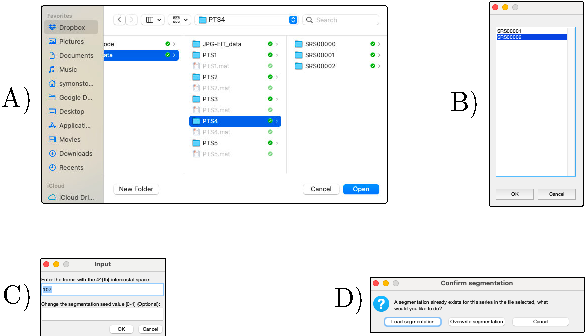
\includegraphics[width=\textwidth]{chapter5-CT_to_mesh/imgs/SegmentationAppSetup.pdf}
	\caption[Manual segmentation data loading]{\label{fig:seg_load}%
	The data loading stages for the manual segmentation program are shown above.
	A) A folder of patient data is selected. B) The desired CT data series is selected.
	C) The initial segmentation frame of the 4\textsuperscript{th} intercostal space 
	is loaded from the patient settings file or input by the user. Optionally, an 
	adjustment to the initial segmentation thresholding value can be input if the 
	segmentation steps failed to locate ribs in the CT image. D) If an existing
	segmentation was saved, the user is asked before a new segmentation 
	is made.
	}
\end{figure}

If an error was made during manual correction, the user could undo
the last change or revert the selected point to the original location. 
Keyboard shortcuts were assigned to each of the functions to reduce the time required
to segment each slice.

\Fref{fig:seg-app-loaded} shows an example of the Matlab GUI for manually correcting
the automatic segmentation. To segment, the user would click \emph{Edit Segment} 
then select and move each point that required correction. The first click by the user
selected the nearest point, and the subsequent click placed the point at the new location. 
Buttons on the side allowed the user to 
select the vertical CT slice for correction, save the segmentation, and generate a mesh. 

\begin{figure}[H]
	\centering
	% Use the following line with your images (pdf preferred)
	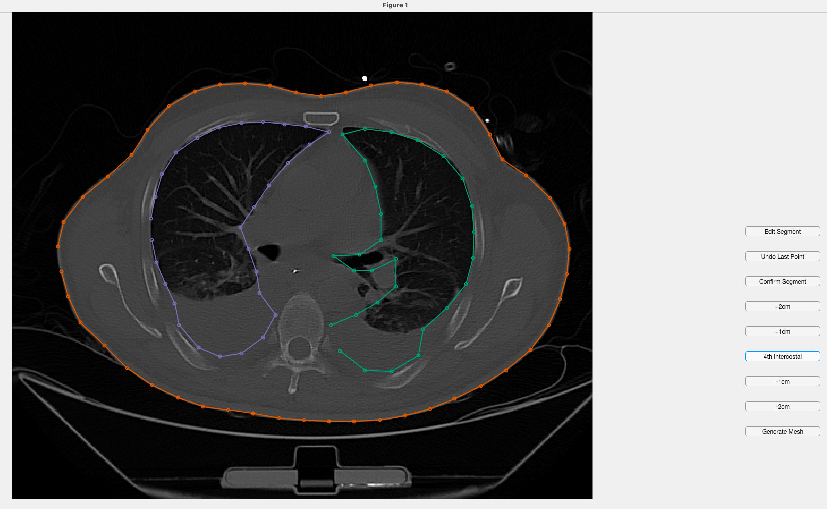
\includegraphics[width=\textwidth]{chapter5-CT_to_mesh/imgs/SegmentationAppLoaded.pdf}
	\caption[Manual segmentation interface with initial input]{\label{fig:seg-app-loaded}%
	An example of a segmentation after being loaded into the segment editor program. 
	The buttons on the right show the options available to the user, and the left shows the 
	CT image for the corresponding slice with the automatic segmentation overlaid.
	}
\end{figure}

After moving each point, an arrow was drawn between the original and new location of the
point last moved to indicate the change and allow the user to see if the
placement was correct. An example of a corrected slice showing the indicating arrow 
is shown in \fref{fig:seg-app-corrected}.

\begin{figure}[H]
	\centering
	% Use the following line with your images (pdf preferred)
	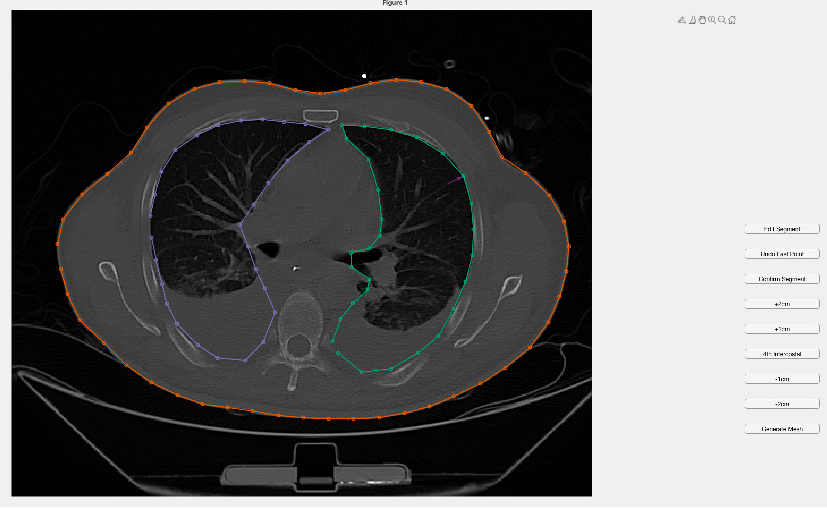
\includegraphics[width=\textwidth]{chapter5-CT_to_mesh/imgs/SegmentationAppCorrected.pdf}
	\caption[Manually corrected segmentation]{\label{fig:seg-app-corrected}%
	An example of a manually corrected segmentation with the arrow indicating the initial
	and new location of the last moved point. The selected point was moved for illustrative
	purposes and was not based on the initial segmentation.}
\end{figure}

The end result was a GUI that allowed for correction and verification of the automatic segmentation 
results. Spatial information from the DICOM image was also saved so that meshes could be
designed to have the correct dimensions and be correctly configured to the patient's size.

\subsection{Mesh Generation} \label{sec:mesh-gen}
There is currently no available tool to automatically generate 3D meshes for 
EIT image reconstruction from a set of points, so the model was simplified using an extrusion technique. 
The \verb!mk_extruded_model! 
function~\parencite{grychtol_fem_2013}
in EIDORS v3.10~\parencite{adler_eidors_2017} was used to extrude the boundary 
of a single segmentation to a height of 20 cm.
The segmentation corresponding to the 4\textsuperscript{th} intercostal space was used for extrusion.
The lungs were specified 2 ways, the first method extruded 2D lung boundaries to form a 3D 
lung region, 
and the second specified a 3D lung boundary  that varied over the height of the model based on the segmentation results.  
To create an accurate 3D lung, we selected all elements of the extruded mesh contained within an 
alpha shape representation of the lung segmentation with an alpha value of 2 cm.

To generate a generic mesh for comparison the \verb!mk_library_model! function in 
EIDORS was used which has available geometry for a cylindrical model with lung regions
and a generic model of a human thorax. The conductivity of the lung regions was set to 
70\% of the background model conductivity.

All images were reconstructed using GREIT for 2D
imaging ~\parencite{adler_greit_2009}. For the GREIT 
reconstructions the noise figure weighting was set to 0.5, 
and 500 targets with a radius of 5 cm were used for training.

\subsection{Evaluation on ARDS Patients} \label{sec:gi-scores}

Diagnostic CT images were acquired from the 
intensive care unit (ICU)
at the Sichuan Provincial People's Hospital
in Chengdu, China.
The research was approved
by the Ethics Committee of Sichuan Academy 
of Medical Sciences \& Sichuan Provincial People's Hospital
(protocol \#201617). 

Diagnostic CT data was acquired from 4 male 
patients aged 39--74 who were diagnosed with ARDS.
EIT data were recorded using the Draeger EIT system on all patients
with a 2D arrangement of 16 electrodes placed at the 
4\textsuperscript{th} intercostal space. 
All patients were mechanically ventilated
at the time of recordings, but the exact 
ventilation parameters are unknown.

To evaluate the effect of the custom models on lung sensitivity,
the centre of mass was computed for both the ventilated region detected in 
CT images, and the breath volume reconstructed in CT images. 
The centre of mass was calculated from EIT images by removing all 
positive changes in the image, then locating the centre of mass 
of all pixels that were greater than 50\% of the ventilation signal amplitude. 
The breath used for the calculation was an ensemble average
of all breaths in the recording.
The error in the centre of mass was calculated between the EIT reconstructed breath 
and the CT segmentation, in number of pixels.
In this chapter a pixel represents between 0.5-2cm depending on the patient size. 

%The GI index was also calculated
%between the generic and custom models with 2D extruded geometry.
%The GI index was calculated using the method
%presented by Zhao et al.~\cite{zhao_evaluation_2009} 
%using the lung regions from the 
%forward model. 
%An estimate of ventilated lung area ($A_V$) relative to the 
%total lung area was calculated from the CT images  
%by dividing the area of the total lung over the ventilated
%lung area 
%(\fref{eq:ventilated_lung_est}).
%\begin{equation}\label{eq:ventilated_lung_est}
%	A_V = \frac{A_{\text{ventilated lung}}}{A_{\text{total lung}}}
%\end{equation}
%
%This was used to determine if the calculated index
%followed the same trend as the percentage of total lung
%that was ventilated in the CT image.
%The GI index was not calculated for the cylindrical model due 
%to the poor reconstruction accuracy, and the 3D lung model was 

\section{Results}

The goal of the automatic segmentation algorithm was to 
generate segmentations that were accurate and could be 
manually verified. \Fref{fig:lung-seg-results}
shows the result of the automatic segmentation regions.
The red overlay indicates the healthy lung segmentation,
and the orange overlay indicates regions that were added
using the estimation method. 
The lungs were examined visually to determine 
how much manual correction was required. During testing
we found this level of accuracy was sufficient to 
complete manual segmentation correction for each subject in 
under 1 minute.

\begin{figure}[H]
	\centering
	% Use the following line with your images (pdf preferred)
	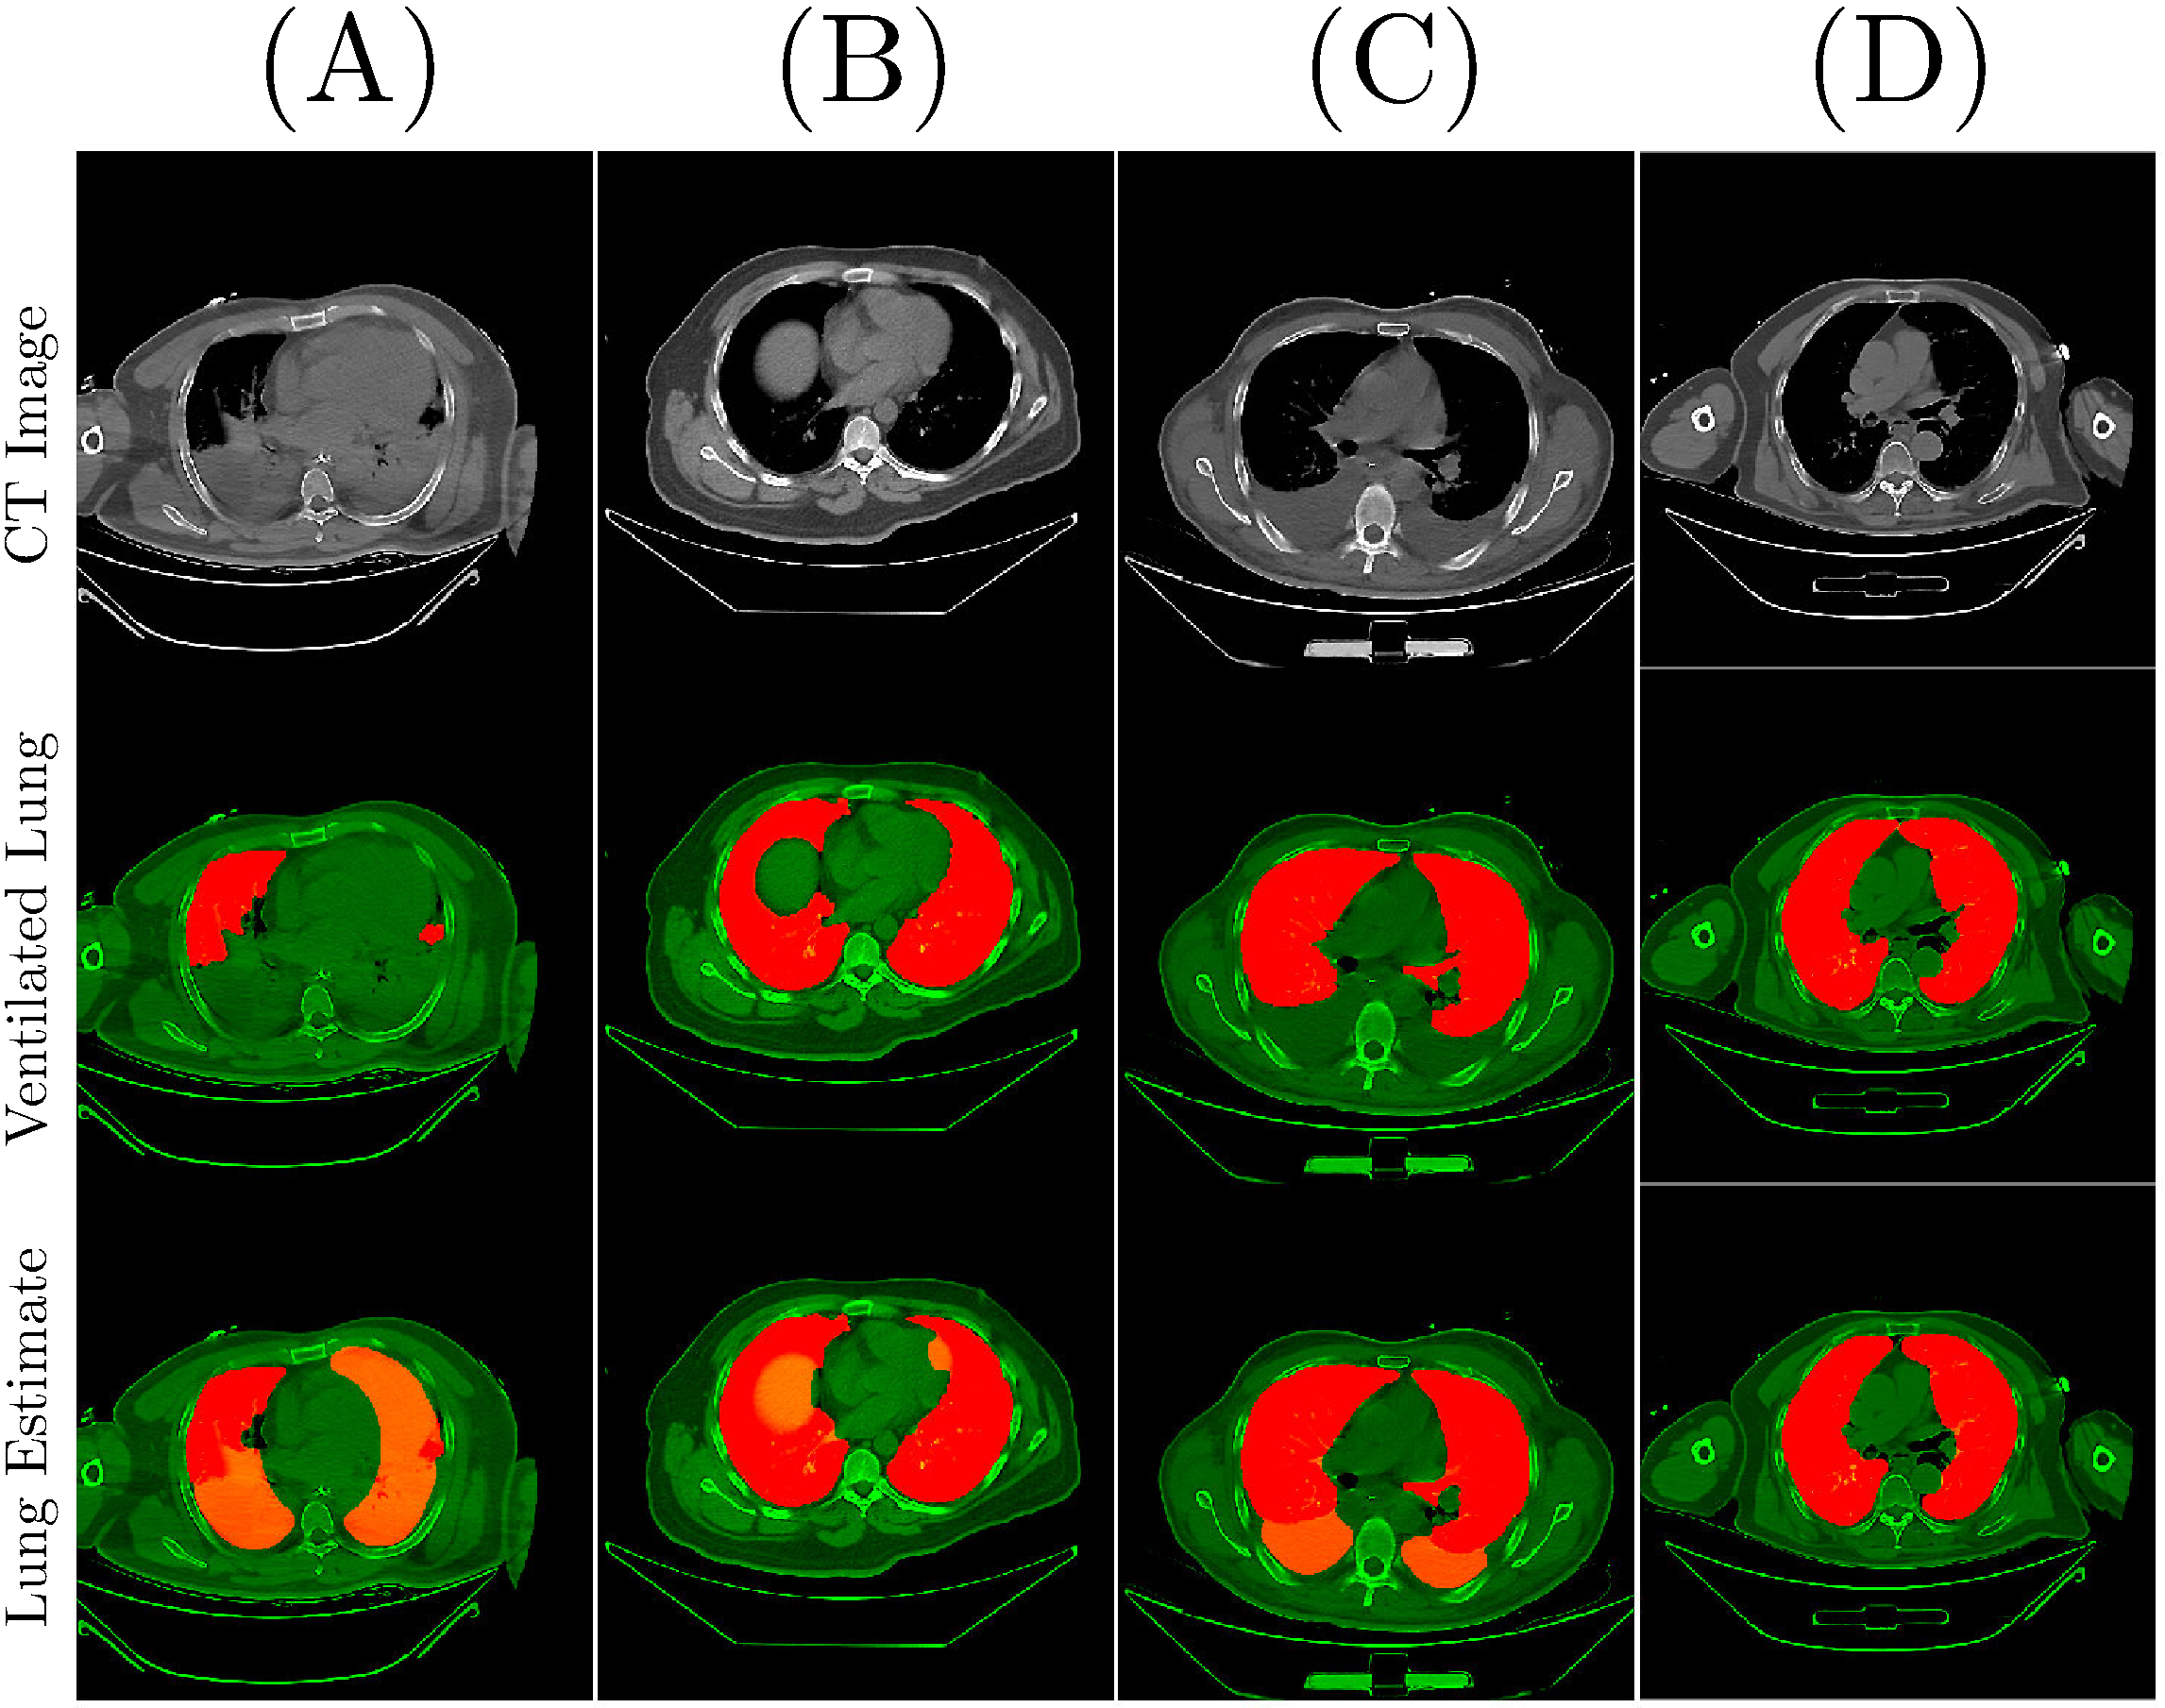
\includegraphics[width=\textwidth]{chapter5-CT_to_mesh/imgs/lung_segmentation_results.pdf}
	\caption[Lung segmentation results]{\label{fig:lung-seg-results}%
	This figure shows the results of the automatic segmentation algorithm. The letters A--D 
	represent the 4 patients. Patient A had a significant portion of the lung that was not
	ventilated, so an estimate was required to obtain lung regions. The ventilated lung estimate
	is shown in red on the 2\textsuperscript{nd} and 3\textsuperscript{rd} columns.
	The total lung area determined using the chest cavity and ventilated lung area is shown in the
	bottom row.}
\end{figure}

The segmentation results show good identification of the
ventilated lung region from the automatic segmentation. The estimated lung regions also helped to 
give starting approximations for the lungs to decrease required manual 
correction time when there was limited ventilated lung in the available CT image.
Sample meshes generated from the segmented images are shown in \fref{fig:fem-results} 
for subject C (in \fref{fig:lung-seg-results}).

\begin{figure}[H]
	\centering
	% Use the following line with your images (pdf preferred)
	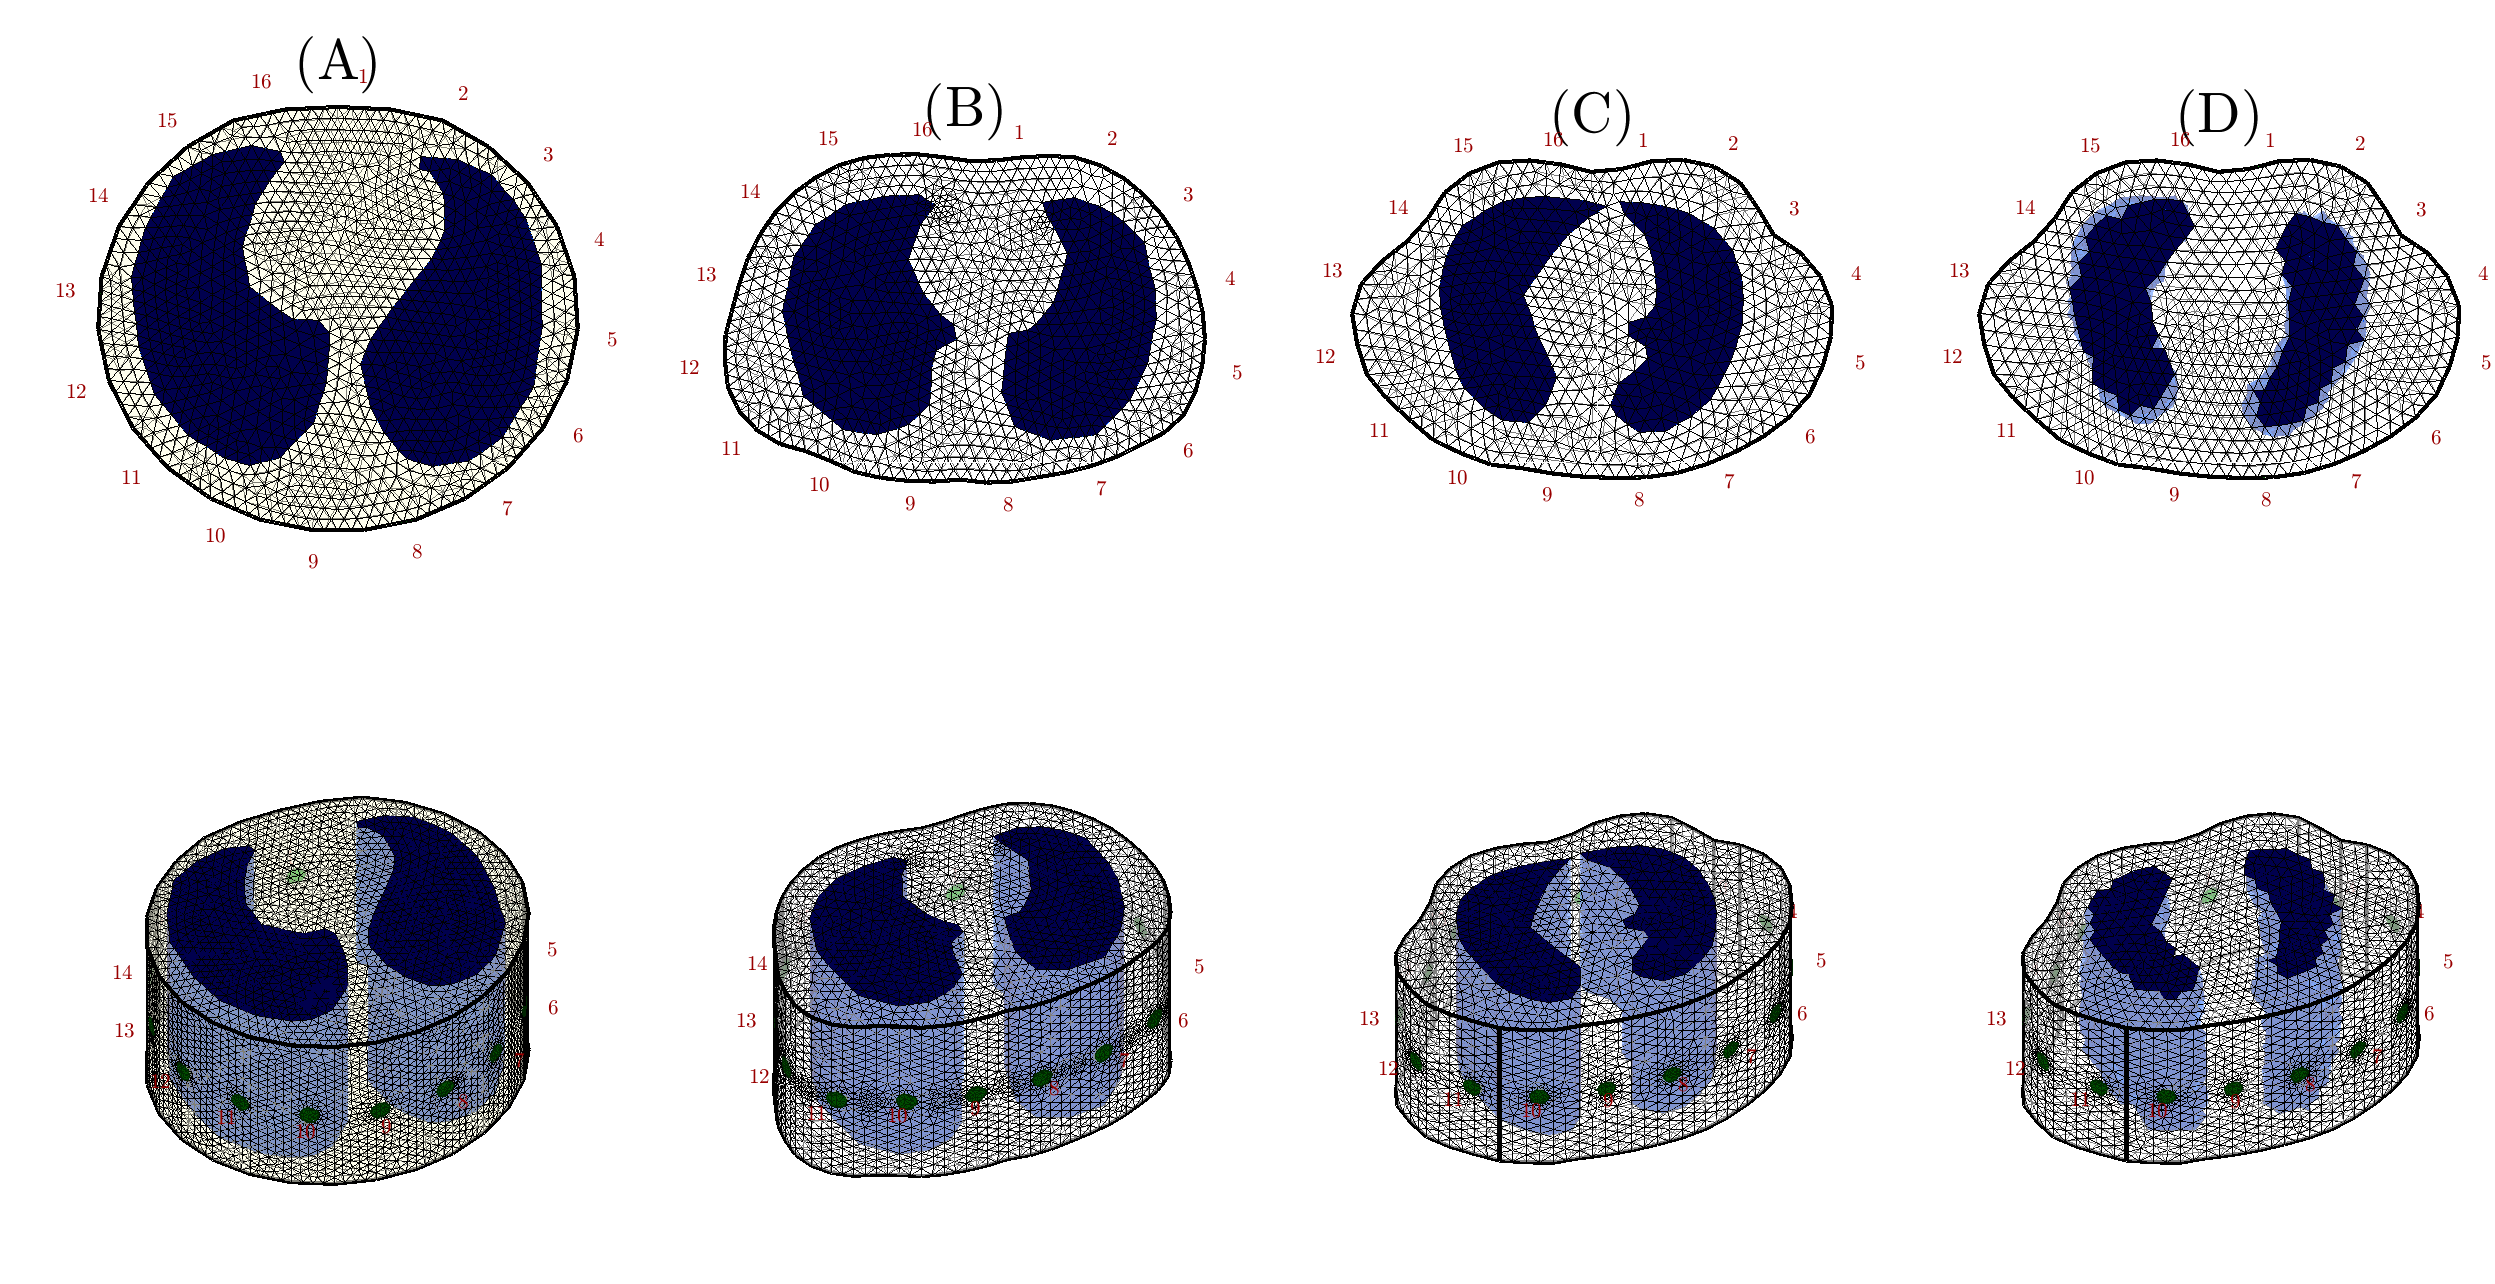
\includegraphics[width=\textwidth]{chapter5-CT_to_mesh/imgs/fem_models_PT04.pdf}
	\caption[Custom and generic meshes]{\label{fig:fem-results}%
	Example meshes and electrode locations for subject C (from \fref{fig:lung-seg-results}).
	Model (A) is cylindrical with lung regions. Model (B) uses the generic chest model from EIDORS. 
	Models (C) and (D) use the custom segmentation boundaries. Model (C) uses 2D lung boundaries 
	from the 4\textsuperscript{th} intercostal space extruded for the model height. Model (D) selects all elements
	are within the 3D lung boundary, as identified by the segmentation results.
	}
\end{figure}

For each patient there was a single EIT recording ranging from 30 -- 60 seconds 
in length.
The ventilation pattern 
from the CT image was compared to the reconstructed ventilation 
on 4 types of models.
The 4 types of meshes compared are pictured in \fref{fig:fem-results}. The first mesh was
cylindrical with approximate lung regions, the second mesh was a generic model 
for an adult thorax, and the final two meshes were created from the segmentations. 
To compare the performance across all models, the centre of mass  was 
compared between the CT-imaged ventilation and the EIT-imaged ventilation.
The mesh with 3D extruded lung regions resulted in a mesh that most closely matched 
the segmentation, since selecting a complex 3D lung region caused some of the
spatial information from the lung segmentation to be lost.

Reconstructed images in \fref{fig:c-of-m-results_a}, 
\fref{fig:c-of-m-results_b},
\fref{fig:c-of-m-results_c} and
\fref{fig:c-of-m-results_d}
show a small difference in ventilated regions 
and centre of mass between custom and generic models. There is a 
noticeable change in ventilation distribution using the circular model, but the 
generic thorax model and the custom models show very similar results. 
There is also a slight shape difference in the ventilation distribution between the generic thorax model 
and custom models, but there is little measurable difference. 

\begin{figure}[H]
	\centering
	% Use the following line with your images (pdf preferred)
	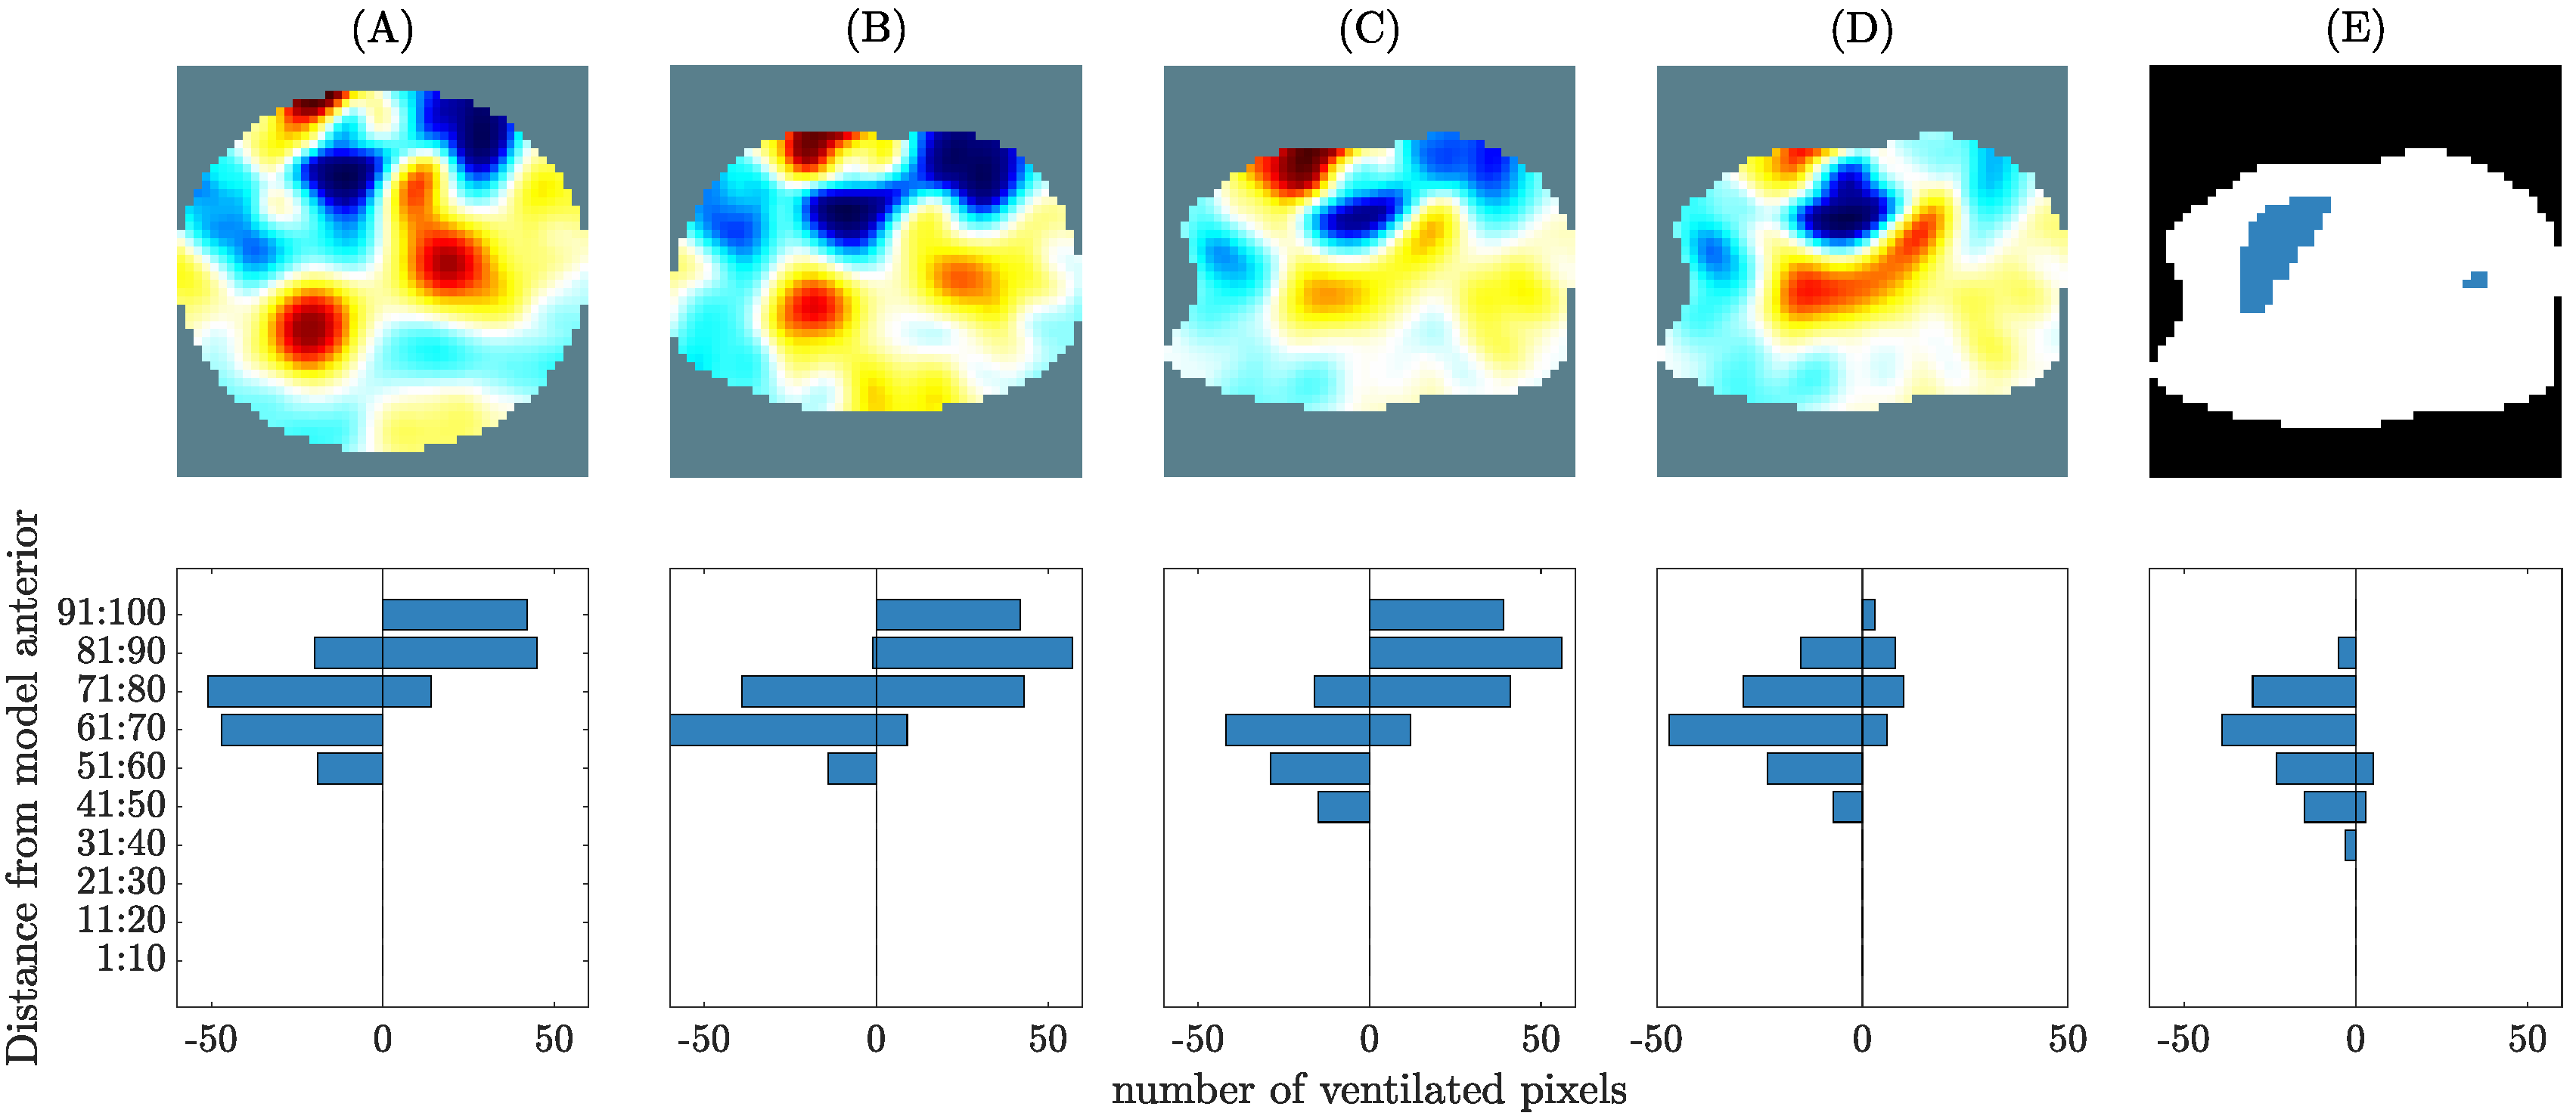
\includegraphics[width=\textwidth]{chapter5-CT_to_mesh/imgs/center_of_vent_PT02.pdf}
	\caption[Example ventilation distributions A]{\label{fig:c-of-m-results_a}%
	Example ventilation distribution for subject A (from \fref{fig:lung-seg-results}).
	Column A and B are the generic models from the EIDORS library. 
	Columns C and D show the custom models with extruded 3D lungs (C) and complex 3D lung regions (D).
	Column E shows the distribution of the ventilated lung as segmented from the CT image. 
	}
\end{figure}

\begin{figure}[H]
	\centering
	% Use the following line with your images (pdf preferred)
	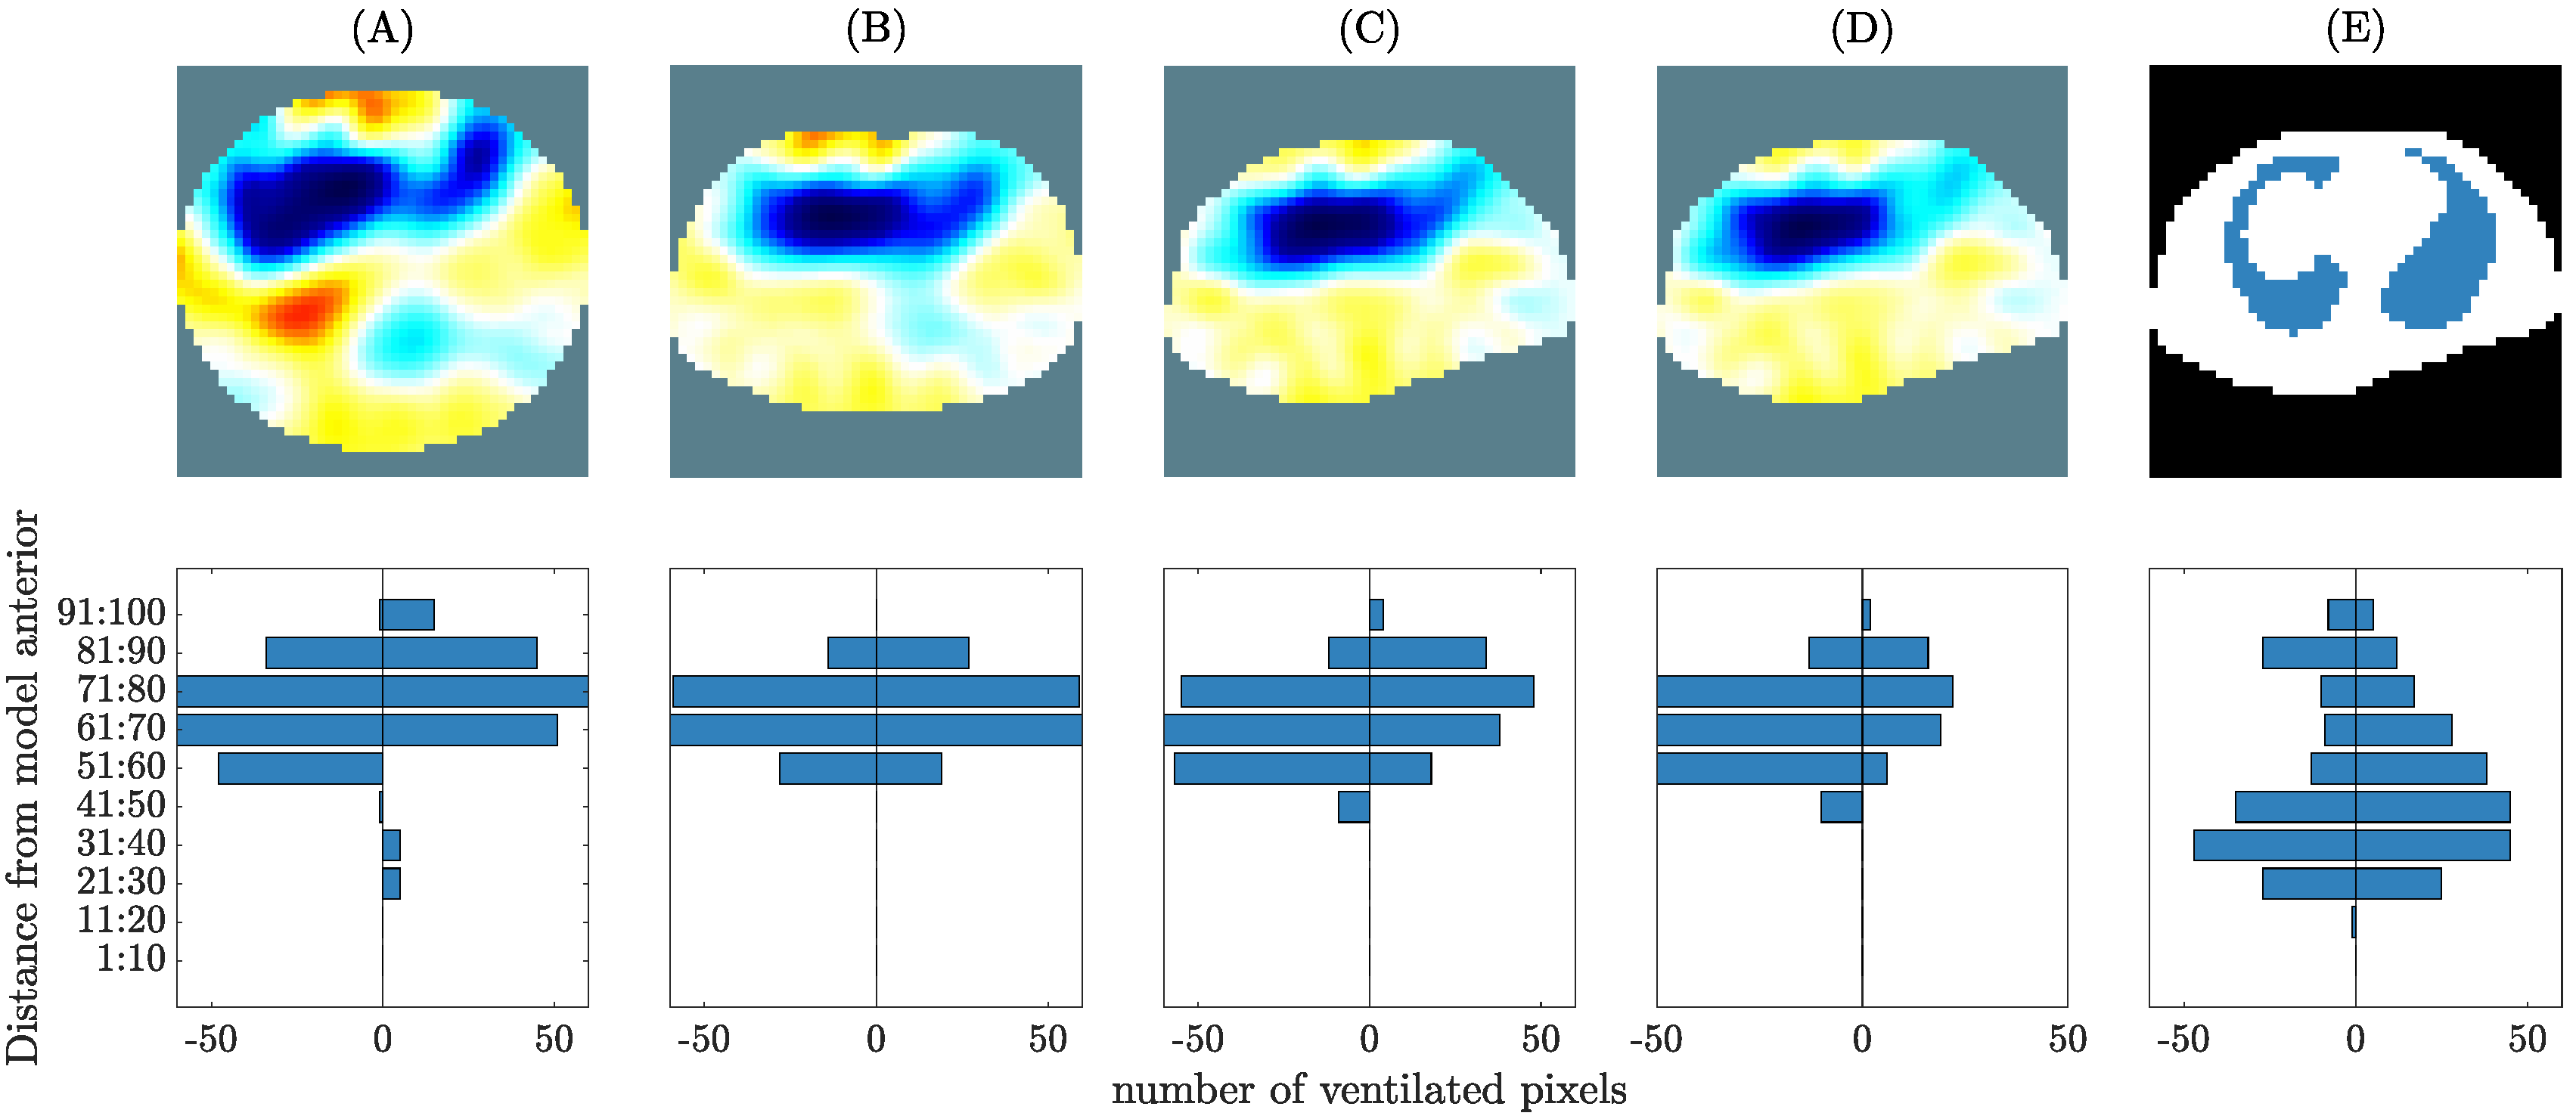
\includegraphics[width=\textwidth]{chapter5-CT_to_mesh/imgs/center_of_vent_PT03.pdf}
	\caption[Example ventilation distributions B]{\label{fig:c-of-m-results_b}%
	Example ventilation distribution for subject B (from \fref{fig:lung-seg-results}).
	Column A and B are the generic models from the EIDORS library. 
	Columns C and D show the custom models with extruded 3D lungs (C) and complex 3D lung regions (D).
	Column E shows the distribution of the ventilated lung as segmented from the CT image. 
	}
\end{figure}

\begin{figure}[H]
	\centering
	% Use the following line with your images (pdf preferred)
	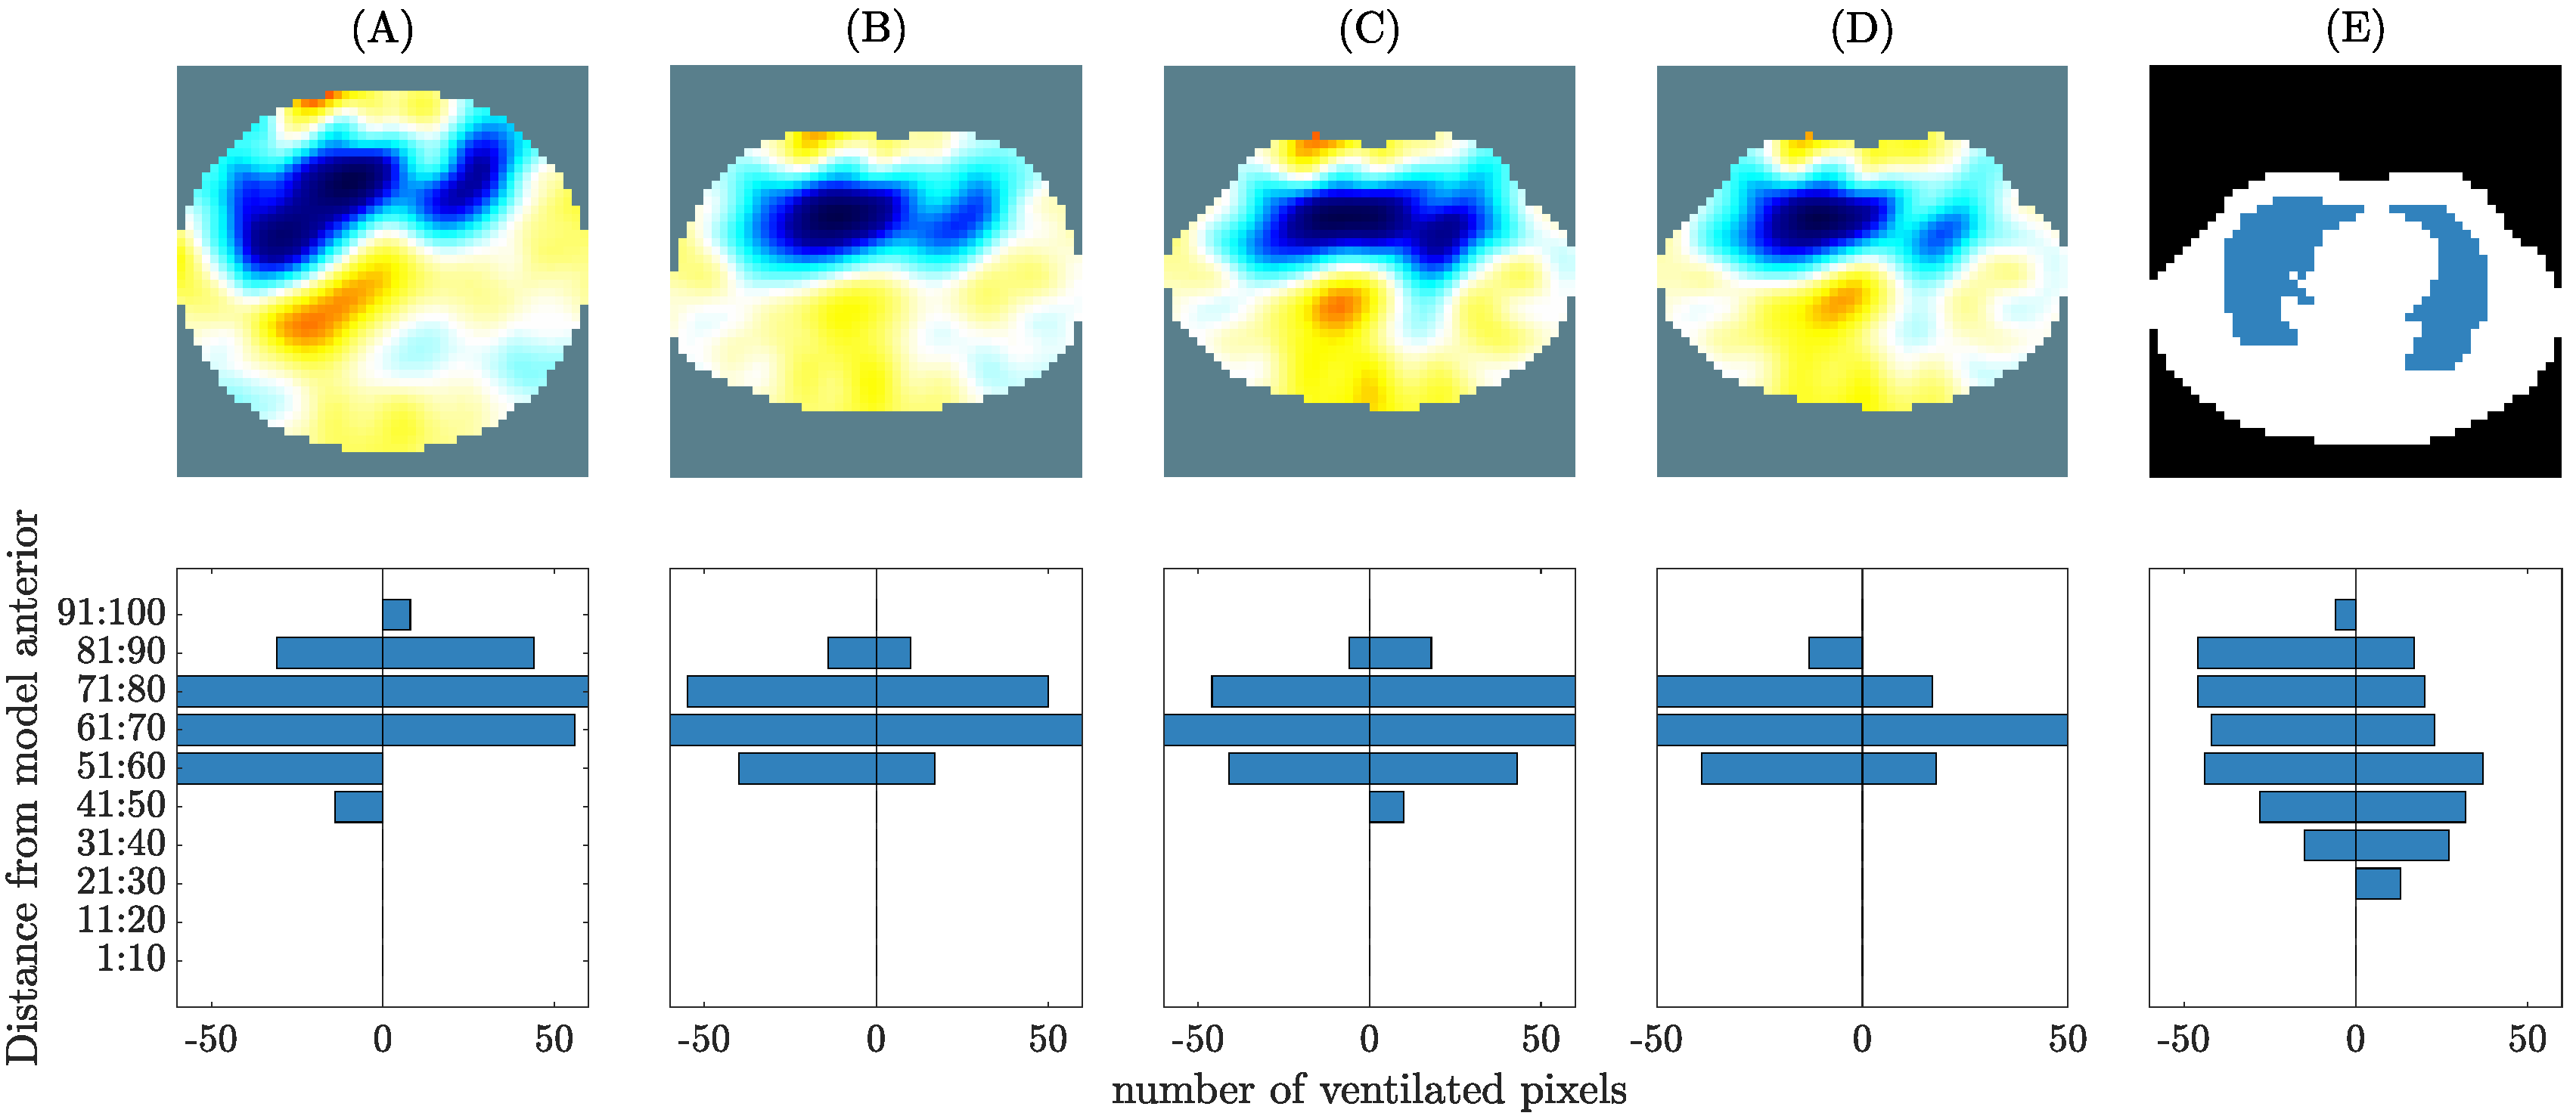
\includegraphics[width=\textwidth]{chapter5-CT_to_mesh/imgs/center_of_vent_PT04.pdf}
	\caption[Example ventilation distributions C]{\label{fig:c-of-m-results_c}%
	Example ventilation distribution for subject C (from \fref{fig:lung-seg-results}).
	Column A and B are the generic models from the EIDORS library. 
	Columns C and D show the custom models with extruded 3D lungs (C) and complex 3D lung regions (D).
	Column E shows the distribution of the ventilated lung as segmented from the CT image. 
	}
\end{figure}

\begin{figure}[H]
	\centering
	% Use the following line with your images (pdf preferred)
	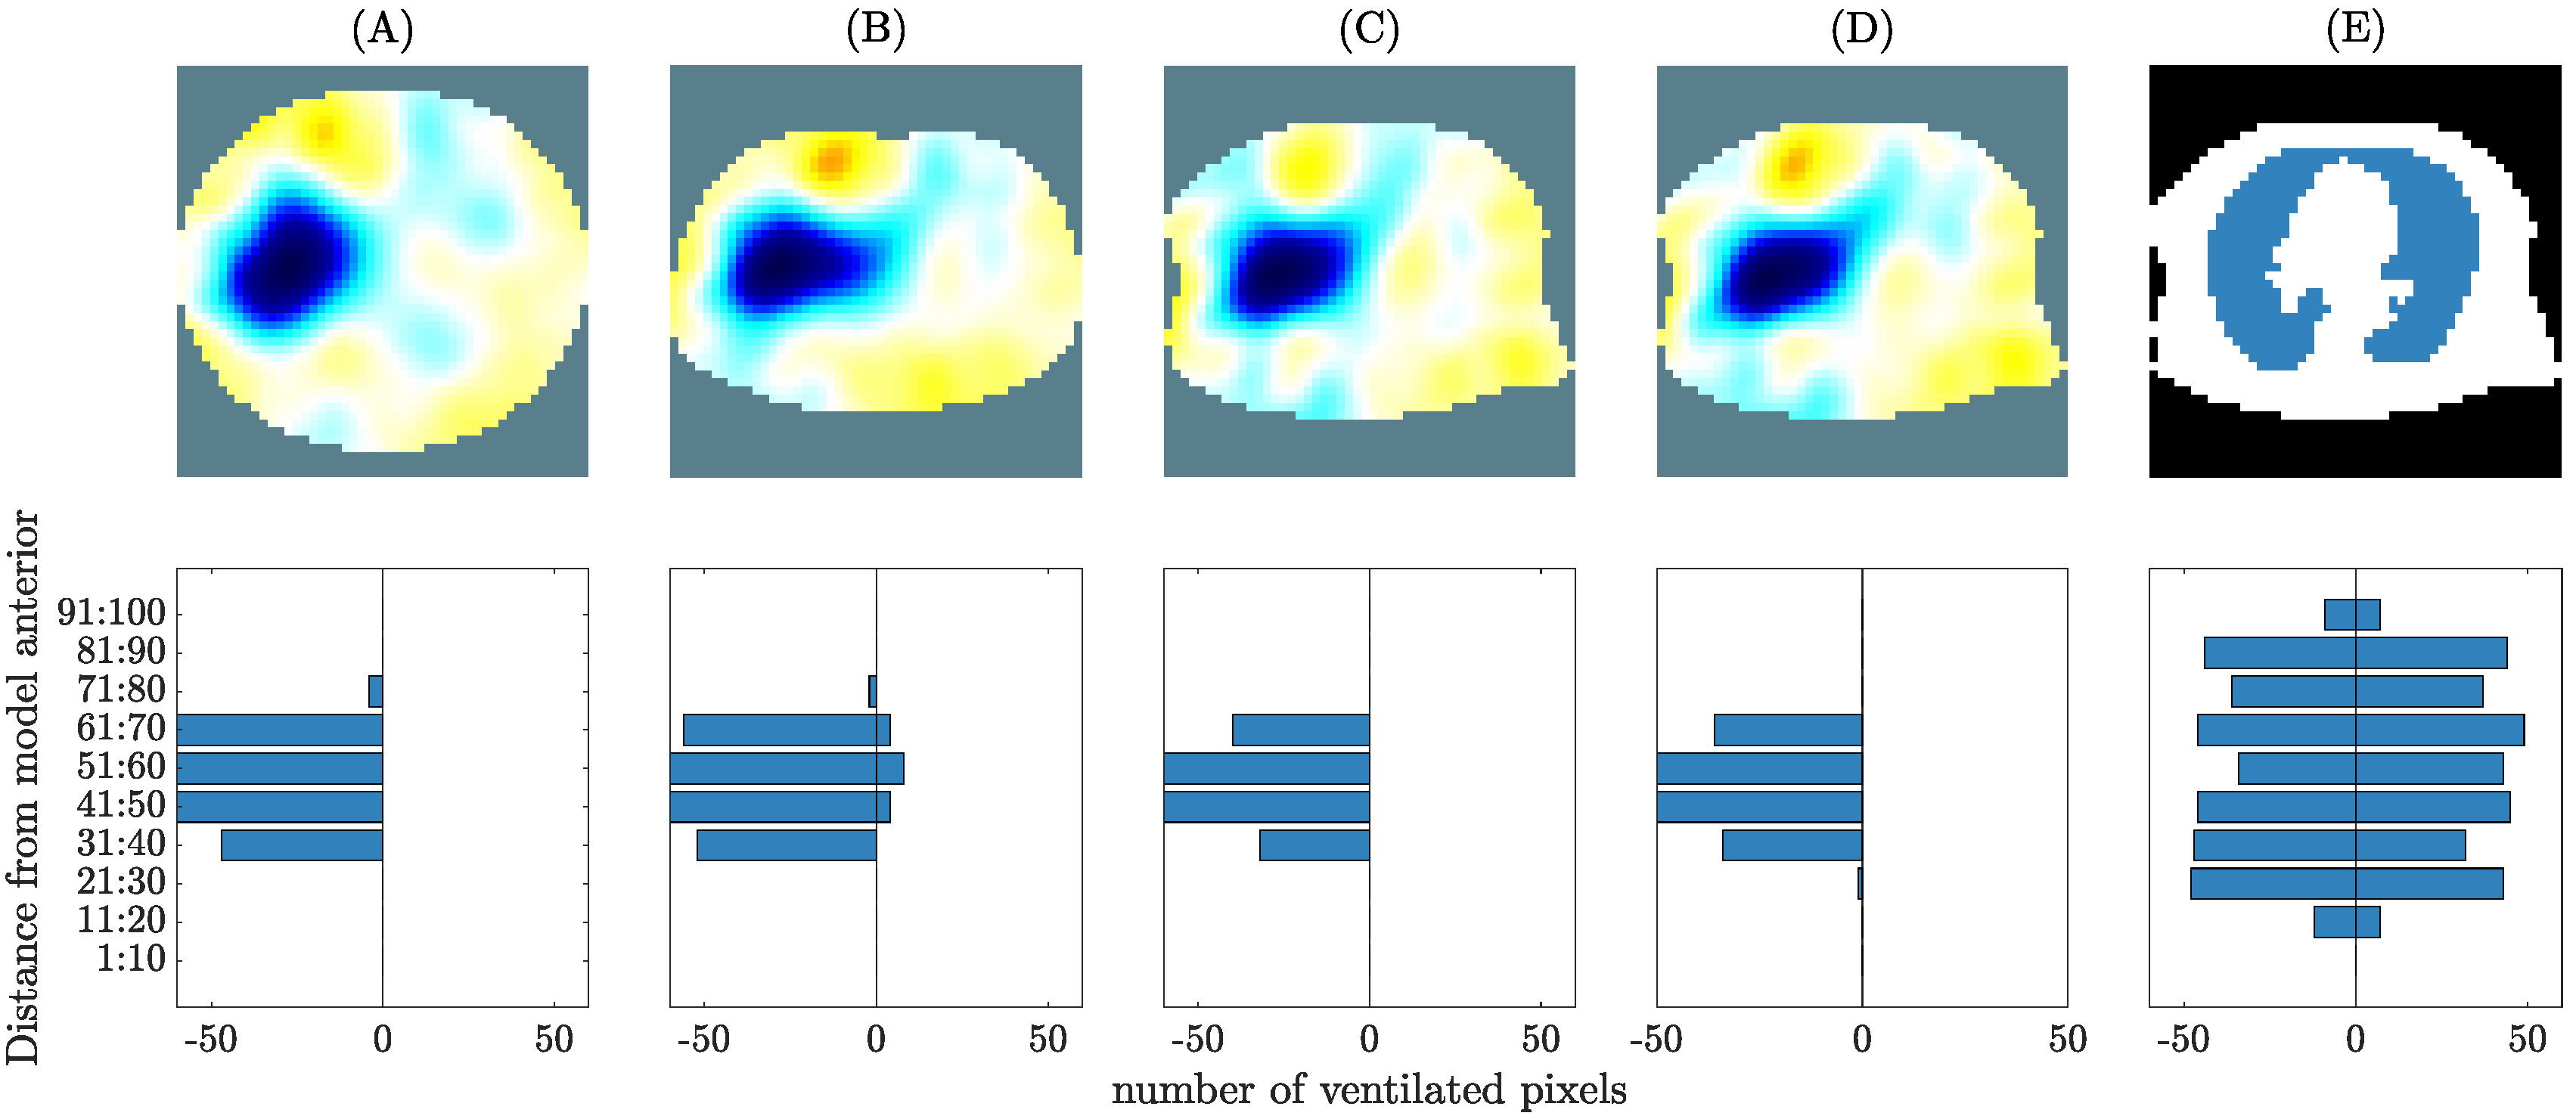
\includegraphics[width=\textwidth]{chapter5-CT_to_mesh/imgs/center_of_vent_PT05.pdf}
	\caption[Example ventilation distributions D]{\label{fig:c-of-m-results_d}%
	Example ventilation distribution for subject D (from \fref{fig:lung-seg-results}).
	Column A and B are the generic models from the EIDORS library. 
	Columns C and D show the custom models with extruded 3D lungs (C) and complex 3D lung regions (D).
	Column E shows the distribution of the ventilated lung as segmented from the CT image. 
	}
\end{figure}


Error in the centre of mass was calculated across all models for each subject 
as shown in \fref{fig:c-of-m-error}. 
The error is estimated as the distance in pixels 
between the centre of mass of the ventilated lung from the CT estimate and the 
centre of mass of the reconstructed breath. 

\begin{figure}[H]
	\centering
	% Use the following line with your images (pdf preferred)
	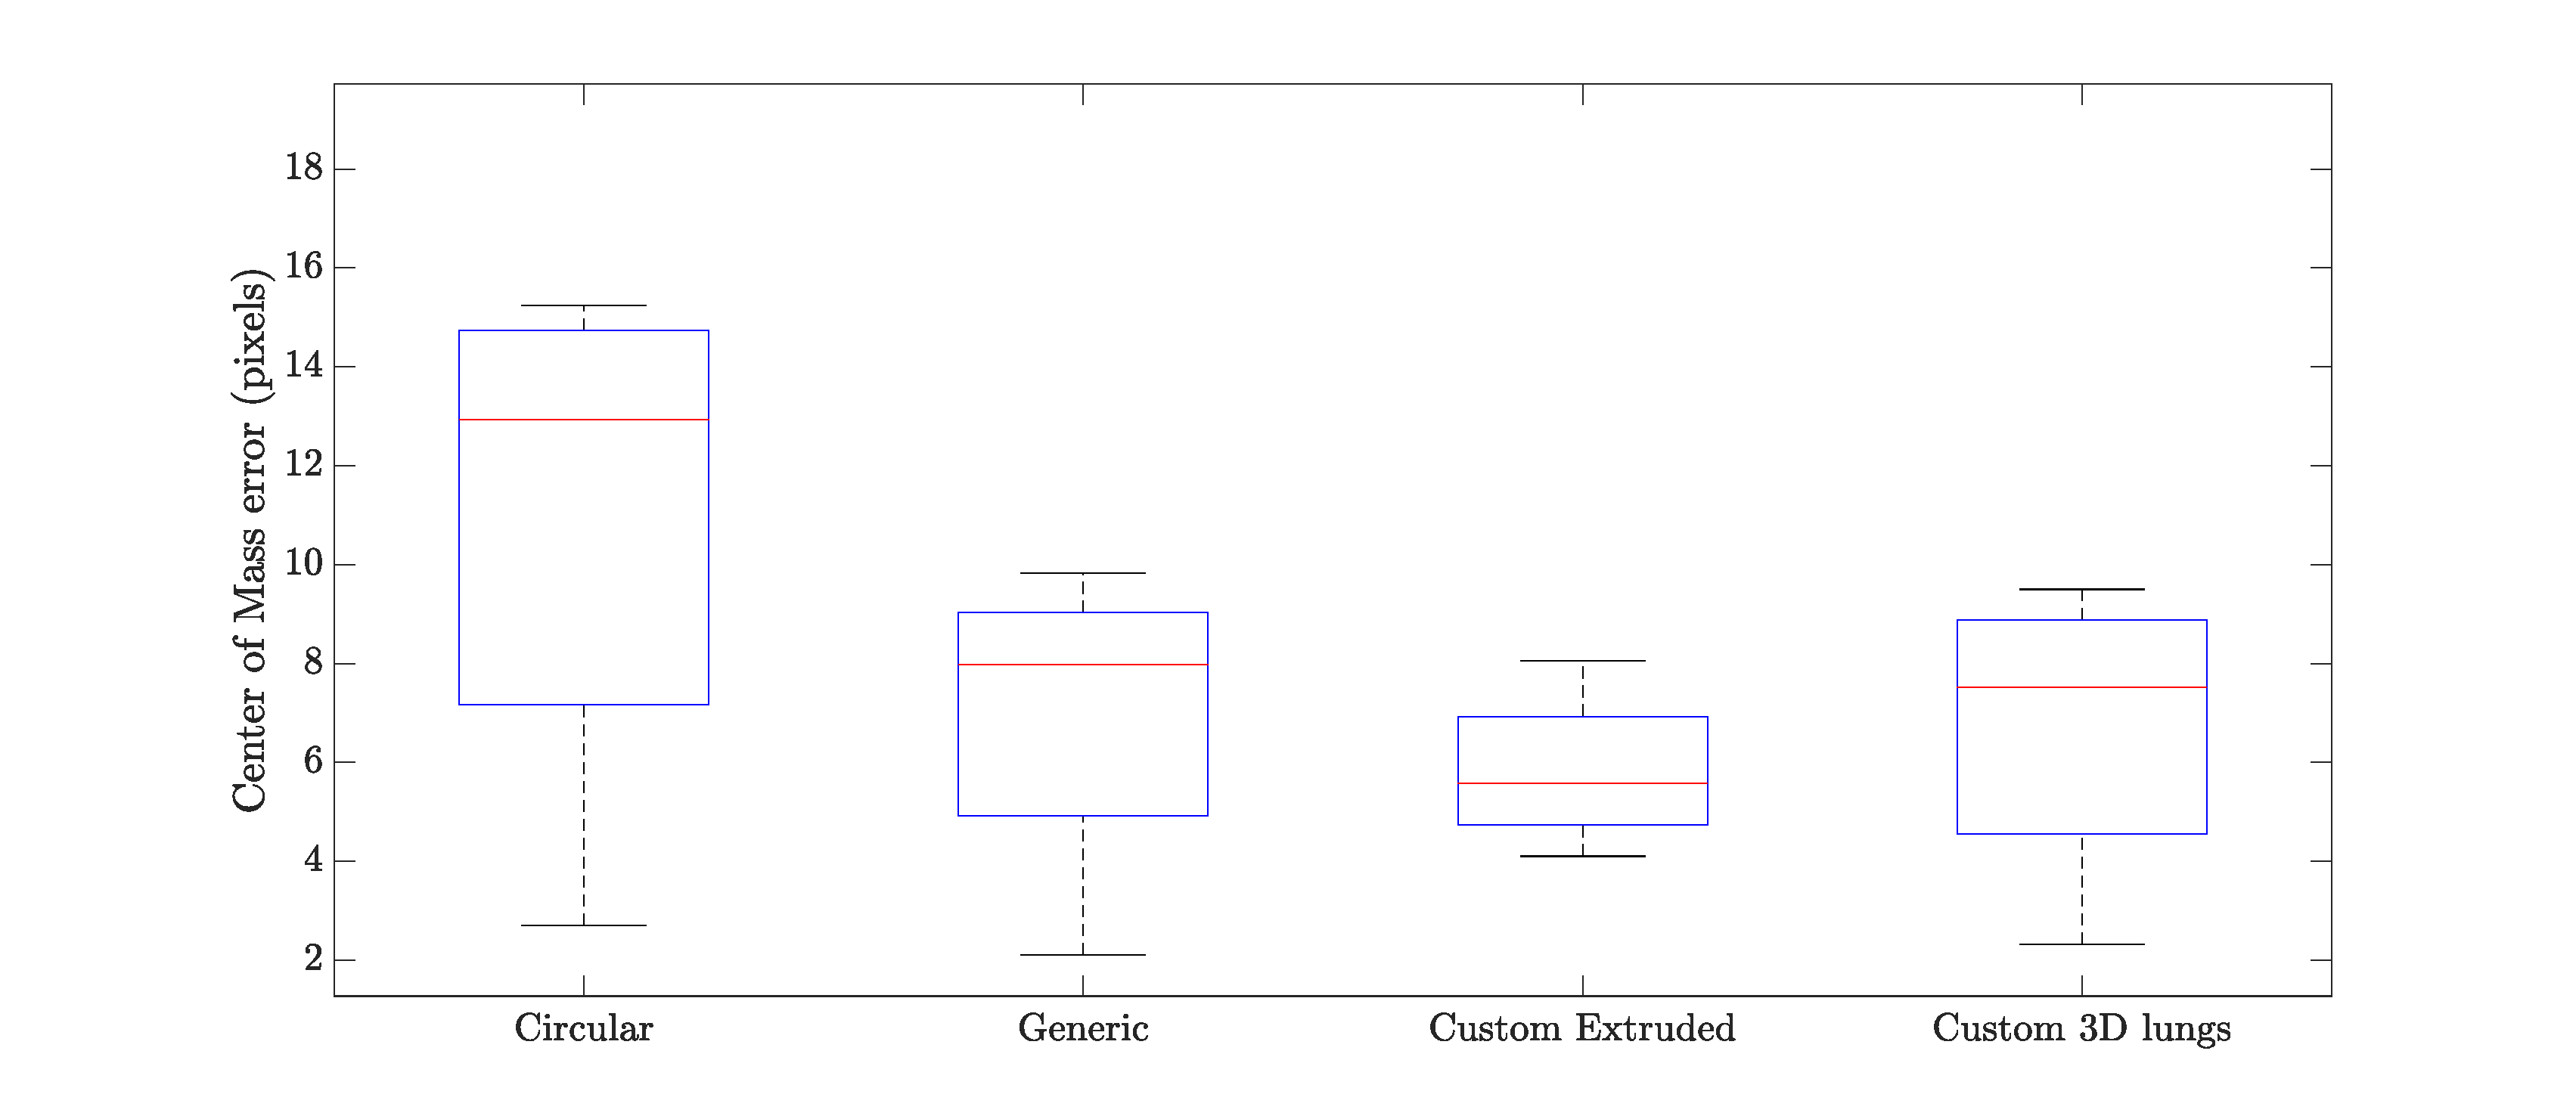
\includegraphics[width=\textwidth]{chapter5-CT_to_mesh/imgs/error_boxplot.pdf}
	\caption[Center of mass error]{\label{fig:c-of-m-error}%
	This figure shows error in the centre of mass measured in pixels for each of the 4 model types investigated.
	From left to right are the circular, generic, 3D extruded, and complex 3D lung region models. 
	One pixel represents between 0.5-2cm depending on the patient and CT configuration.
	}
\end{figure}

Based on this small sample size it seems that the custom extruded models show some improvement 
over generic EIT models. 
All body-shaped models performed better than the cylindrical model 
as measured by error in the centre of ventilation,
and there was little difference between the generic model and the model with complex 3D lung regions. 
%The centre of mass error was not significantly different across all models for each of the subjects. 
%The average error for the circular model was slightly higher than the customized geometry, but for 
%all models the centre of mass, and shape of the ventilation distribution was similar. It is not clear 
%that custom models improved reconstruction accuracy of breath reconstructions in the EIT images. 
There are several potential factors that could contribute to the similarity in performance across
most models. 

\section{Discussion}
The goal of this chapter was to create a tool to automatically segment CT images 
to improve lung reconstruction accuracy. 
We believe this may help to enhance individualized ventilation monitoring for ARDS patients. 
An automatic segmentation algorithm was developed to give a baseline segmentation of the lungs which 
gave an approximate starting point for the true lung boundary. A tool for manual correction was designed 
that enabled quick, accurate corrections of automatically generated CT images. 
Segmented images were used to generate meshes with accurate boundary  shapes and lung outlines. 

%Although it has been shown that accurate models of the boundary and lung improve measures of
%GI index~\parencite{yang_lung_2021}, the models with improved boundary accuracy in this chapter 
%did not show this improvement. 
Previous studies looked at the effect of model accuracy on GI index and found that a more 
accurate body surface and lung boundary improved results \parencite{yang_lung_2021}. 
The results presented here show only a small improvement when examining difference in  the centre
of ventilation. A large sample size is required to determine if the improvement is consistent.
One factor that was different between the two studies was the value 
of lung conductivity. \citeauthorandyear{yang_lung_2021} used a conductivity value of 1.3 times the background conductivity for the lung 
tissue. This is atypical since the conductivity of lung tissue is 
considerably lower than other tissues in the body. 
In this chapter a lung conductivity of 70\% of the 
background conductivity was
used. Using a value of 
1.3 times the background 
conductivity did not decrease the centre of mass error across custom models.
There was also a difference in the centre of ventilation error when comparing 
between both custom models. One potential reason is that when selecting the elements that were
contained within the complex 3D lung regions, the boundary of the lungs was distorted slightly and a less accurate
representation of the lungs was given. 
If images were acquired with a 3D arrangement of electrodes, the use of a complex 3D volume to represent the lungs 
could have more of an effect.

There are several other factors that may contribute to the mismatch between the 
CT ventilation and the EIT imaged ventilation. 
First, the difference in posture and condition between the CT and the EIT image 
was not known. The EIT belt was not in position during the CT scan, so  there was potential that the
patient position and posture were slightly changed. Although this may contribute to a slightly different
shape of the thorax, it is not likely to drastically change the boundary of the chest cavity. 
One of the larger factors is likely the unknown locations of the electrodes. Since the exact location 
of the electrode is unknown, the 16 electrodes were  places evenly around the thorax in the model. 
Modelling the electrode locations incorrectly can have a large impact on the resulting EIT
image, causing artefact and lower reconstruction accuracy \parencite{boyle_impact_2011}.
Since the CT images acquired 
contain spatial information, there is potential to improve accuracy of the 
electrode placement on the models. The EIT system that was used has several available belts with 
different electrode spacing and points of attachment. If the user was able to select 
the belt used and the electrode spacing in the software, 
the electrode locations could be more accurately
approximated. Alternatively, an image or CT with the electrode belt in place could allow
precise estimation of the electrode location and spacing. It may also 
be feasible to reconstruct the electrode location partially using a movement jacobian 
\parencite{soleimani_imaging_2006}, although it is not currently possible to do this 
with the GREIT algorithm. 

In addition to improving the accuracy of electrode placement in the meshes,
there is still future development 
planned for the segment editor and automatic segmentation. Initial tests were done on the CT and EIT data
from 4 patients, and validation across a wider dataset is required to ensure stability 
of the automatic segmentation and ease of editing. Improvements to the appearance of the interface and 
documentation must also be added before the software is easy to use in a clinical setting. 
Work is currently underway to obtain several more sets of CT and EIT data to validate the automatic 
segmentation and manual correction steps. Once the number of patients is increased, 
the project will use these meshes to build a library of meshes that can be extended for 
use on patients without CT. A library of meshes coupled with machine learning based on physical 
attributes could allow for custom meshes to be used on patients even when no CT data is available. 

When using the complex 3D lung region model, there was a
slight reduction in the amplitude of a conductive artefact that appeared in the centre of
the images. It is possible that the 3D aspect of the model allows the 3D path of the current
to be modelled more accurately~\parencite{adler_electrical_2017}, but the 
extent of the benefit is limited when using a 2D arrangement of 
electrodes~\parencite{grychtol_3d_2016}. The segmentation techniques could be used to 
create an even further customized model with different conductivity regions assigned to 
fluid in the lungs and collapsed regions. While this could give more spatially accurate 
reconstructions, we still do not expect a high degree of spatial accuracy using EIT. The 
advantage of EIT is primarily the high temporal resolution. Additionally, 
the collapsed regions and liquid in the lung may move over time. Identifying the entire lung 
region allows us to track changes in impedance within the lung region.

When creating meshes using the \verb!ng_mk_extruded_model! in EIDORS \parencite{grychtol_fem_2013}, 
accurate models with a good representation of the boundary are created, but 
Netgen occasionally fails to mesh the electrodes on models. We presume this is 
due to irregular and concave curves.
This occurred several times on the segmented data, so a more robust meshing
or electrode placement technique will be required. Placing complex 3D lung boundaries helped to reduce 
errors that were introduced by tight corners on lung segmentations, but electrode and boundary meshing
errors were still present in this model. 

\section{Summary}

The diagnostic CT images required for ARDS patients are an excellent source of spatial 
information about the size and location of organs in a subject. 
A segmentation and 
boundary-editing tool
was developed to generate accurate meshes of the external and lung
boundaries from CT images. 
The custom meshes with an extruded boundary show a slight reduction in error 
when comparing centre of ventilation to the CT images.
In ARDS patients with very poor lung health, segmentation of the actual lung boundary is 
challenging. However, with a multi-step process including automatic segmentation and 
manual verification, we generated accurate customized meshes for 
a small number of ARDS patients. 
Small benefits were observed when reconstructing ventilation images 
on custom meshes, and additional steps to improve the modelled electrode 
locations could help to further improve reconstructions. 
Work is currently underway to validate and improve the segmentation tool on 
a larger dataset of ARDS patients. 
Methods to reduce the impact of sensitivity to electrode 
location error on reconstructions, or correctly identify 
correct electrode locations could help to further improve this technique. 

%\TODO{Delete the rest of this?}
%Data from 4 ARDS patients with CT
%and EIT were used to develop a segmentation 
%and correction tool to identify 
%the lungs and boundary of the body.  
%Segmentation was done using the 4th intercostal space, 
%with 10 adjacent CT 
%slices to form an enclosed chest cavity. 
%The lungs
%and exterior boundary were identified by increasing the contrast
%and identifying an appropriate threshold.
%Each segmentation was downsampled to
%20 points that could be edited by the user in Matlab. The 
%mesh was generated using 
%\verb!ng_mk_extruded_model!~\cite{Grychtol2012} in EIDORS 
%3.10~\cite{Adler2019}. Images were reconstructed 
%using GREIT~\cite{Adler2009}. 
%
%
%\begin{figure}
%\centering
%% Use the following line with your images (pdf preferred)
%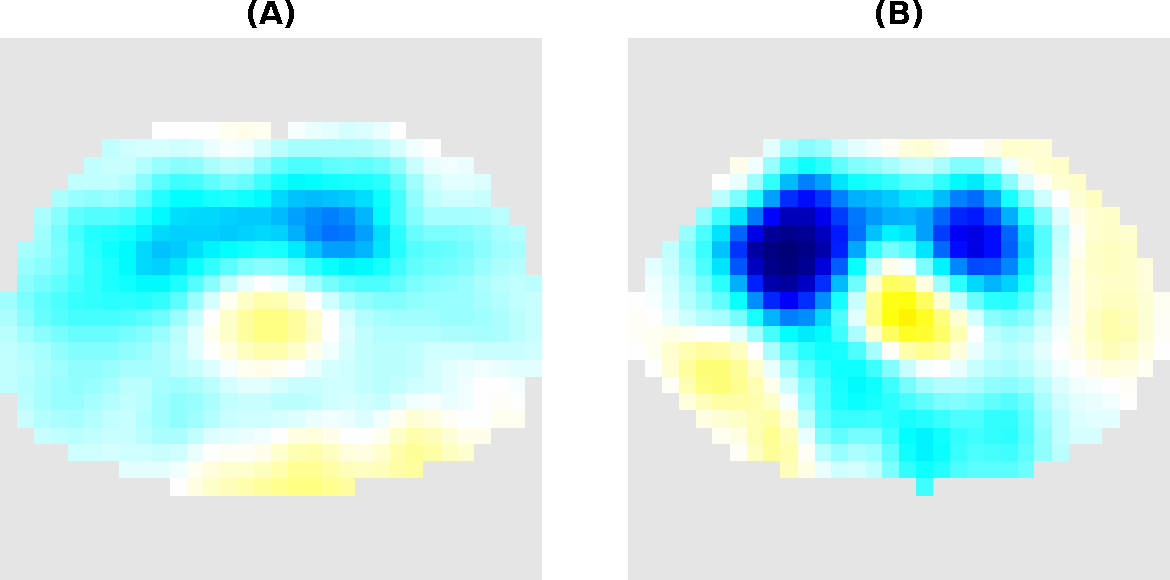
\includegraphics[width=\textwidth]{chapter5-CT_to_mesh/imgs/basic_vs_advanced_3_cropped.pdf}
%\caption{\label{fig:ct_mesh_breath}%
%Single breath using: A) generic model B) custom model
%}
%\end{figure}
%
%Results in figure~\fref{fig:breath} show a reconstructed image 
%with more separable lungs in the enhanced model, and a mean GI index for each breath in the 
%1 minute 
%recording that follows 
%trend of the ventilated lung percentage in table~\ref{tbl:twocol}.
%
%\begin{table}
%  \centering
%  \caption{\label{tbl:twocol} %
%  Ventilated lung estimate vs. GI index scores.}
%  \begin{tabular}{|p{1.2cm}|p{1.5cm}|p{1.8cm}|p{1.7cm}|}
%    \hline
%  Subject & Ventilated lung (\%) &
%  GI (basic model) & GI (custom model) \\ \hline
%  1 & 99.9 & 0.353$\pm$0.004& 0.690$\pm$0.005 \\ 
%  2 & 85.5 & 0.640$\pm$0.022& 0.771$\pm$0.020  \\
%  3 & 79.6 & 0.695$\pm$0.007& 0.857$\pm$0.009  \\
%  4 & 27.0 & 0.614$\pm$0.011&  1.81$\pm$0.053 \\\hline
%  \end{tabular}
%  \vspace{-1em} 
%\end{table}
%
%\section{Discussion}
%
%The goal of this chapter was to design a tool to make custom meshes of 
%
%$\sigma$